\documentclass[aps,prb,twocolumn,superscriptaddress,floatfix,longbibliography]{revtex4-2}

\usepackage[utf8]{inputenc}
\usepackage[spanish]{babel}
\usepackage{graphicx}
\usepackage{amsmath}
\usepackage{subcaption}
\usepackage{wrapfig} 
\usepackage[export]{adjustbox}

\usepackage{amsmath,amssymb} % math symbols
\usepackage{bm} % bold math font
\usepackage{graphicx} % for figures
\usepackage{comment} % allows block comments
\usepackage{textcomp} % This package is just to give the text quote '
%\usepackage{ulem} % allows strikeout text, e.g. \sout{text}

\usepackage[spanish]{babel}

\usepackage{enumitem}
\setlist{noitemsep,leftmargin=*,topsep=0pt,parsep=0pt}

\usepackage{xcolor} % \textcolor{red}{text} will be red for notes
\definecolor{lightgray}{gray}{0.6}
\definecolor{medgray}{gray}{0.4}

\usepackage{hyperref}
\hypersetup{
colorlinks=true,
urlcolor= blue,
citecolor=blue,
linkcolor= blue,
bookmarks=true,
bookmarksopen=false,
}

% Code to add paragraph numbers and titles
\newif\ifptitle
\newif\ifpnumber
\newcounter{para}
\newcommand\ptitle[1]{\par\refstepcounter{para}
{\ifpnumber{\noindent\textcolor{lightgray}{\textbf{\thepara}}\indent}\fi}
{\ifptitle{\textbf{[{#1}]}}\fi}}
\ptitletrue  % comment this line to hide paragraph titles
\pnumbertrue  % comment this line to hide paragraph numbers

% minimum font size for figures
\newcommand{\minfont}{6}

% Uncomment this line if you prefer your vectors to appear as bold letters.
% By default they will appear with arrows over them.
% \renewcommand{\vec}[1]{\bm{#1}}

%Cambiar Cuadros por Tablas y lista de...
%\renewcommand{\listtablename}{Índice de tablas}
\renewcommand{\tablename}{Tabla}
\renewcommand{\date}{Fecha}

\graphicspath{ {C:/Users/lupam/OneDrive/Escritorio/GitHub/IntroCUDA/Final/Script_presentacion/Figures/} } %Para importar imágenes desde una carpeta

\usepackage[bottom]{footmisc} %para que las notas al pie aparezcan en la misma página




\begin{comment}

%Comandos de interés:

* Para ordenar el documento:
\section{Introducción}
\section{\label{sec:Formatting}Formatting} %label para luego hacer referencia a esa sección

\ptitle{Start writing while you experiment} %pone nombre y título al documento dependiendo de si en el header están los comandos \ptitletrue y \pnumbertrue

* Ecuaciones:
\begin{equation}
a^2+b^2=c^2 \,.
\label{eqn:Pythagoras}
\end{equation}

* Conjunto de ecuaciones:
\begin{eqnarray}
\label{eqn:diagonal}
\nonumber d & = & \sqrt{a^2 + b^2 + c^2} \\
& = & \sqrt{3^2+4^2+12^2} = 13
\end{eqnarray}

* Para hacer items / enumerar:
\begin{enumerate}
  \item
\end{enumerate}

\begin{itemize}
  \item
\end{itemize}

* Figuras:
\begin{figure}[h]
    \includegraphics[clip=true,width=\columnwidth]{pixel-compare}
    \caption{}
     \label{fig:pixels}
\end{figure}

* Conjunto de figuras:
(no recuerdo)


* Para hacer referencias a fórmulas, tablas, secciones, ... dentro del documento:
\ref{tab:spacing}

* Para citar
Elementos de .bib
\cite{WhitesidesAdvMat2004}
url
\url{http://www.mendeley.com/}\\

* Agradecimientos:
\begin{acknowledgments}
We acknowledge advice from Jessie Zhang and Harry Pirie to produce Fig.\ \ref{fig:pixels}.
\end{acknowledgments}

* Apéndice:
\appendix
\section{\label{app:Mendeley}Mendeley}

* Bibliografía:
\bibliography{Hoffman-example-paper}

\end{comment}



\begin{document}

% Allows to rewrite the same title in the supplement
\newcommand{\mytitle}{Desarrollo de dispositivos con redes percolativas de nanohilos de plata.}

\title{\mytitle}

\author{Pablo Chehade \\
    \small \textit{pablo.chehade@ib.edu.ar} \\
    \small \textit{Introducción al Cálculo Numérico en Procesadores Gráficos, Instituto Balseiro, CNEA-UNCuyo, Bariloche, Argentina} \\}


\maketitle

Script de la presentación de CUDA


\section{Introducción}
El objetivo del proyecto es simular la dinámica de un gas de N electrones contenido en un recinto circular de radio $R_0$. En particular, nos interesa conocer las propiedades del gas en el equilibrio.

\begin{figure}[h]
    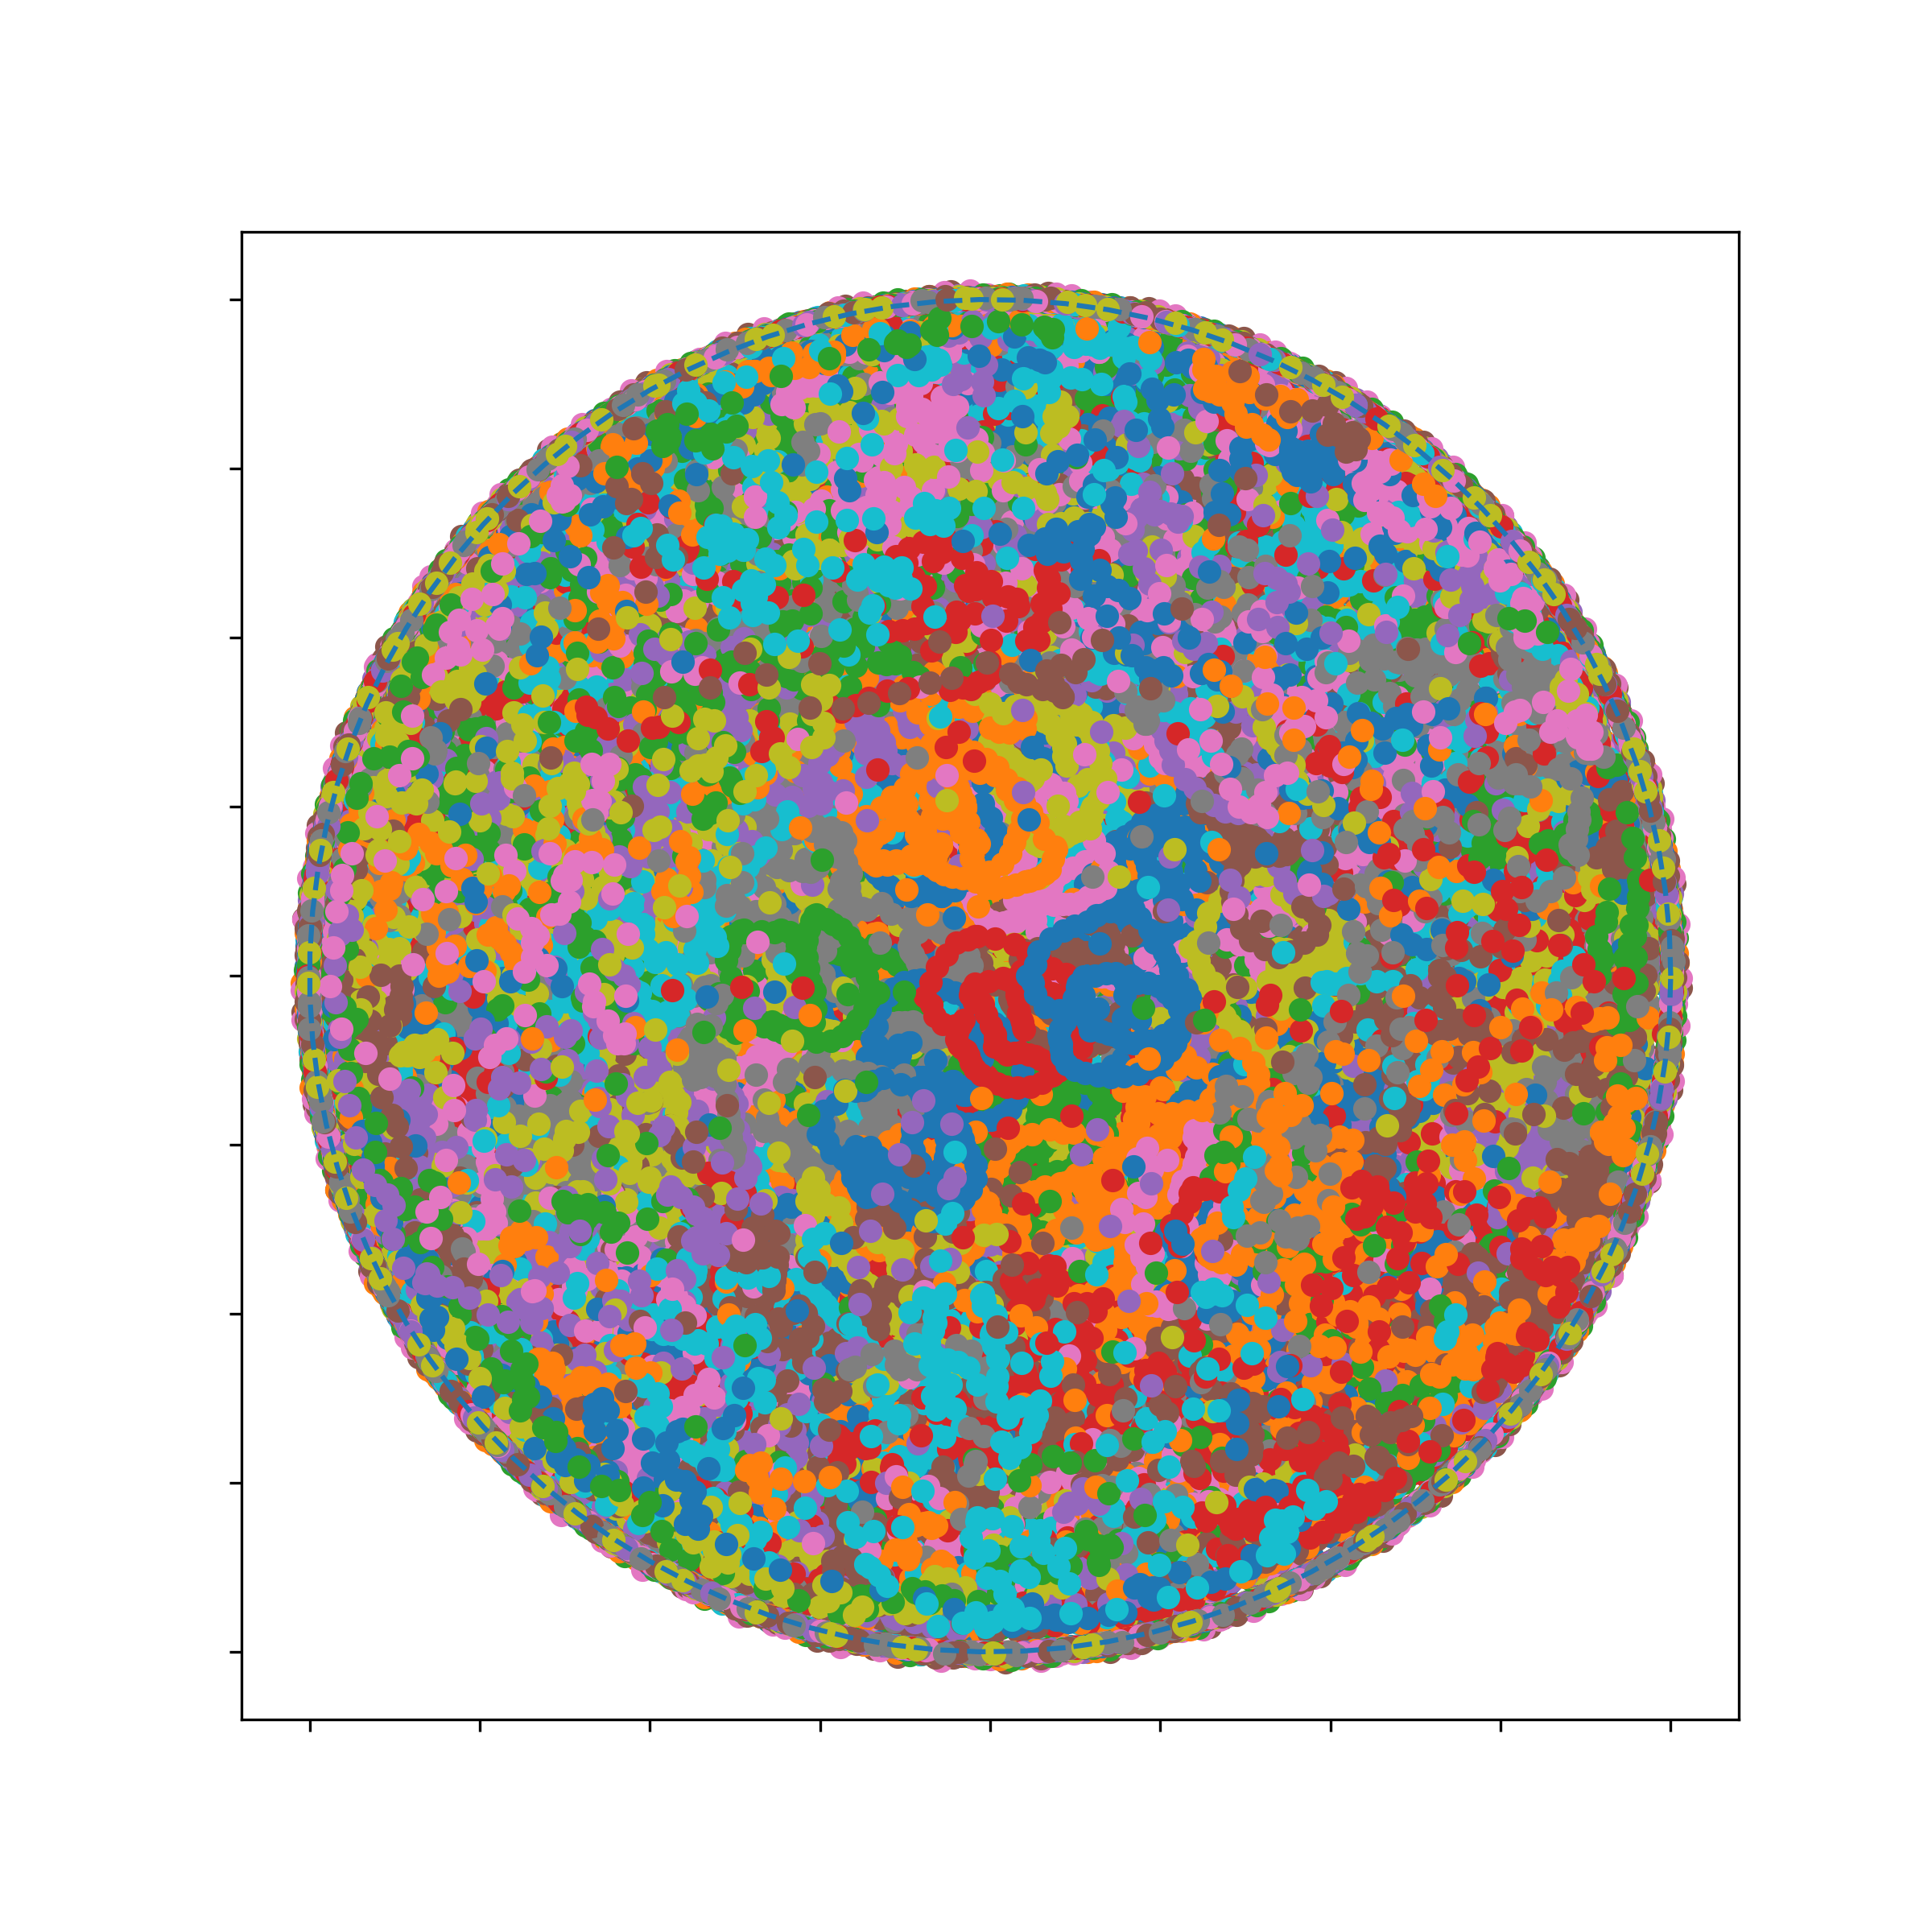
\includegraphics[clip=true,width=\columnwidth]{electrones_en_caja.png}
    \caption{Figura representativa: algunos electrones adentro de un círculo de radio $R_0$. Hacerlo con python y con el mismo formato que los resultados.}
     \label{fig:electrones_en_caja}
\end{figure}






\section{Motivación}
El estudio de estas propiedades permite analizar el proceso de evolución de una avalancha de electrones generada en una cavidad rodeada por una fuente de electrones.


\begin{itemize}
    \item Explicar el proceso de avalancha de electrones de la tesis
\end{itemize}


\section{Definición del problema}

\ptitle{Opciones de modelo y qué modelo elegimos}
Para modelar el gas de electrones hay 2 opciones:
\begin{enumerate}
    \item estadística
    \item partículas
\end{enumerate}


% \begin{figure}[h]
%     \includegraphics[clip=true,width=\columnwidth]{pixel-compare}
%     \caption{}
%      \label{fig:pixels}
% \end{figure}

\subsection{Ecuaciones de movimiento}

\ptitle{Ecuaciones}
ecuaciones de movimiento dadas por la ley de Newton y la ley de Lorentz, adimensionalizadas


\begin{itemize}
    \item \textcolor{red}{Ecuaciones adimensionalizadas}
\end{itemize}

\[\]


\ptitle{Método de Verlet}
\textcolor{red}{Ecuaciones del método}
(método simpléctico? conservativo)

\subsection{Condiciones iniciales}

Como condición inicial se parte de $N$ electrones en posiciones y velocidades aleatorias con distribución uniforme, ambas entre $0$ y $1$ por la adimensionalización elegida.


\[$r_{0,i,x}, r_{0,i,y} \sim U(0, 1)$ \forall i \]
\[$v_{0,i,x}, v_{0,i,y} \sim U(0, 1)$ \forall i \]

\subsection{Corección de Temperatura}

El sistema es conservativo, de modo que dadas las condiciones iniciales la energía se conserva en el tiempo. La energía está constituida por energía cinética (temperatura) y energía potencial. Pero a nosotros no nos interesa el equilibrio para dada energía inicial total, sino que nos interesa el equiñlibrio a determinada temperatura. De este modo, se va a corregir 

\subsection{Colisiones con la pared}

Se asume que las colisiones con la pared son elásticas, considerando la misma como una "pared blanda". Esto significa que durante la evolución la partícula invierte su velocidad si atraviesa la pared, pero no se refleja su posición. Esto es útil para evitar discontinuidades en la energía total del sistema.


\begin{figure}[h]
    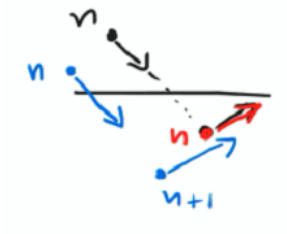
\includegraphics[clip=true,width=0.4\columnwidth]{rebote_blando.png}
    \caption{Figura del rebote blando}
     \label{fig:rebote_blando}
\end{figure}

\section{Método Numérico}

\section{Implementación}



\ptitle{¿Qué pasos debe hacer nuestro código para calcular la evolución del gas de electrones?}

\begin{enumerate}
    \item Loop sobre partículas: asignar aleatoriamente posición y velocidades de las $N$ partículas
    \item Loop temporal:
    \begin{enumerate}
        \item Dadas $r_0^n$ y $v_0^n$ calculas $r_0^{n+1}$ y $v_0^{n+1}$ mediante el método de Verlet. Esto implica
        \begin{enumerate}
            \item Loop sobre partículas: calcular $F_{i,j}^n$
            \item Loop sobre partículas: calcular las nuevas posiciones $r_{i}^{n+1}$
            \item Loop sobre partículas: calcular $F_{i,j}^{n+1}$
            \item Loop sobre partículas: calcular las nuevas velocidades $v_{i}^{n+1}$
        \end{enumerate}
        \item Loop sobre partículas: verificar si alguna partícula "chocó" con la pared, es decir, ver si $|r_0^{n+1}| > R_0$. En caso positivo, invertir la velocidad radial
        \item Loop sobre partículas: corregir las velocidades para que la temperatura sea la deseada
    \end{enumerate}
\end{enumerate}
\textcolor{blue}{Poner los items anteriores. Poner "loop sobre partículas" y "loop temporal" en un color distinto.}

Los procesos son
\begin{itemize}
    \item Condiciones iniciales
    \item Loop temporal
    \begin{itemize}
        \item Método de Verlet
        \begin{itemize}
            \item Cálculo de fuerzas
            \item Integración de posiciones y velocidades
        \end{itemize}
        \item Rebotes
        \item Corrección de velocidades
    \end{itemize}
\ned{itemize}


Condiciones iniciales
Loop temporal
Método de Verlet
Cálculo de fuerzas
Integración de posiciones y velocidades
Rebotes
Corrección de velocidades




Tenemos muchos loops que podrían ser paralelizables

\section{Versiones del código en serie y en paralelo}
*Contar cada versión por separado.
\textcolor{blue}{Hacer una tabla traspuesta en la que diga}

Versión 1	Python	En serie (numpy)
Versión 2	Python	En paralelo (numpy -> cupy)
Versión 3	C++	En serie
Versión 4	CUDA C	En paralelo (kernels)
Versión 5	CUDA C	En paralelo (kernels + shared memory)

Me gustaría hacer una "historia" de cómo fui cambiando de una versión a la otra y en el camino menciono cómo fui haciendo las cuentas. Esto debería intercalarse con el profiling y los gráficos de speed-up

\subsection{Versión 1: Python en serie}

\begin{itemize}
    \item Esta versión fue implementada en un Notebook de Python. Se empleó este lenguaje porque inicialmente el problema no estaba bien definido y tuve que hacer mucho prototyping
    \item Para hacer los cálculos de forma eficiente, decidí usar numpy en lugar de los loops de python.
    \item \textcolor{blue}{Ejemplo de código en el que usé numpy: asignación de las condiciones iniciales}
    \item Pude hacerlo en todos los pasos salvo en el cálculo de los rebotes, ahí usé loops de python
    \item En particular, la consecuencia de lo anterior fue tener que calcular una matriz de fuerzas
    \item \textcolor{blue}{Gráfico de la matriz de fuerzas}
    \item \textcolor{red}{Análisis del tiempo de cómputo}
    \item \textcolor{red}{Análisis de profiling}
\end{itemize}


\begin{figure}[h]
    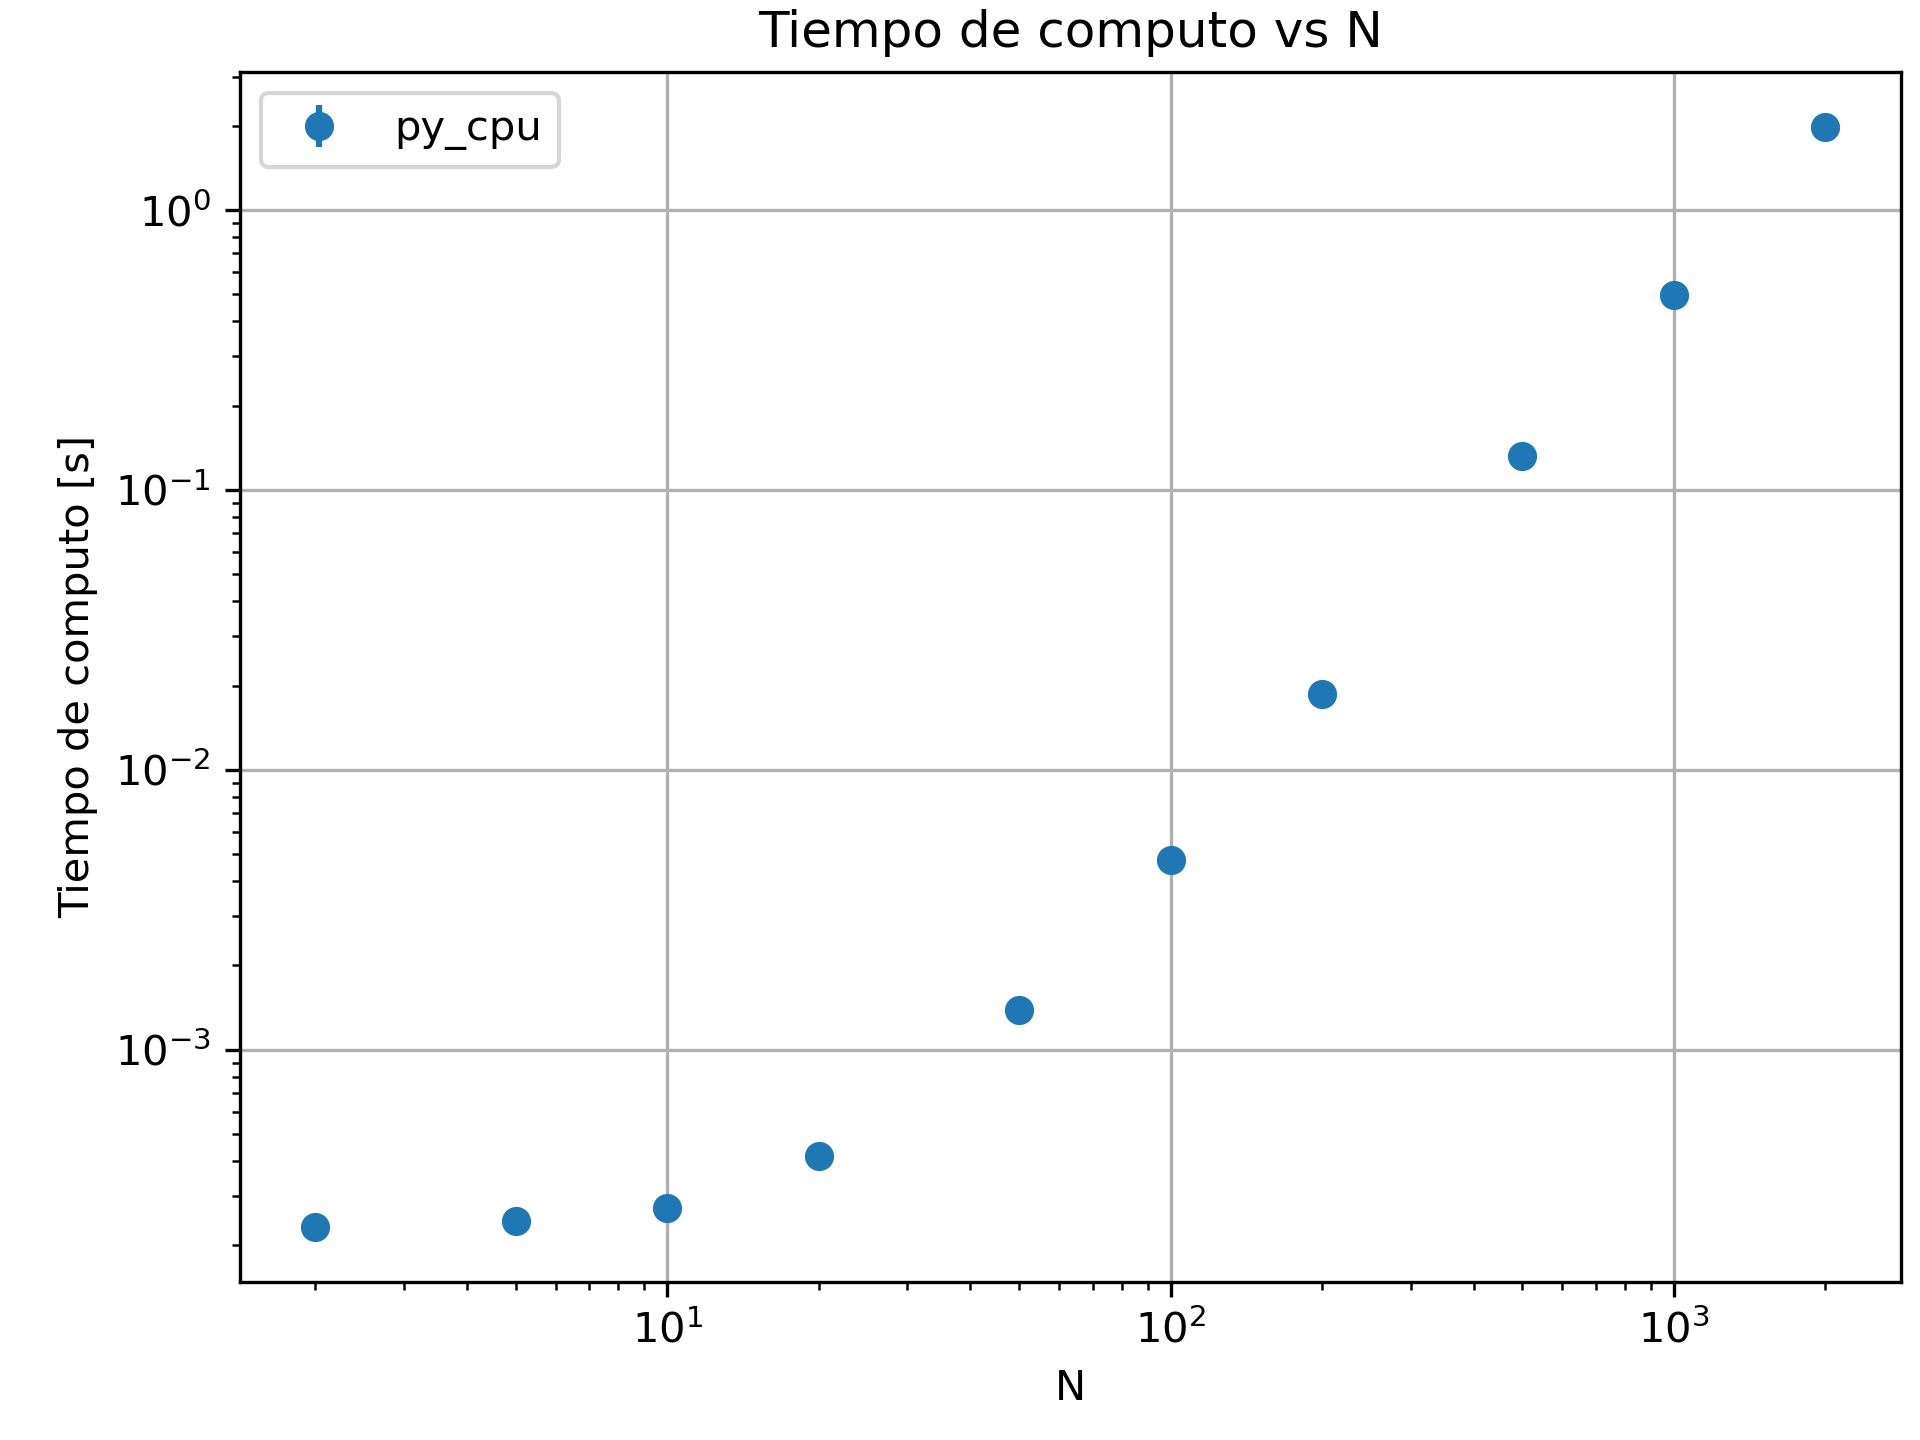
\includegraphics[clip=true,width=\columnwidth]{tiempo_de_computo_vs_N_py_cpu.png}
    \caption{Gráfico de tiempo de cómputo}
     \label{fig:tiempo_de_computo_vs_N_py_cpu}
\end{figure}

\begin{figure}[h]
    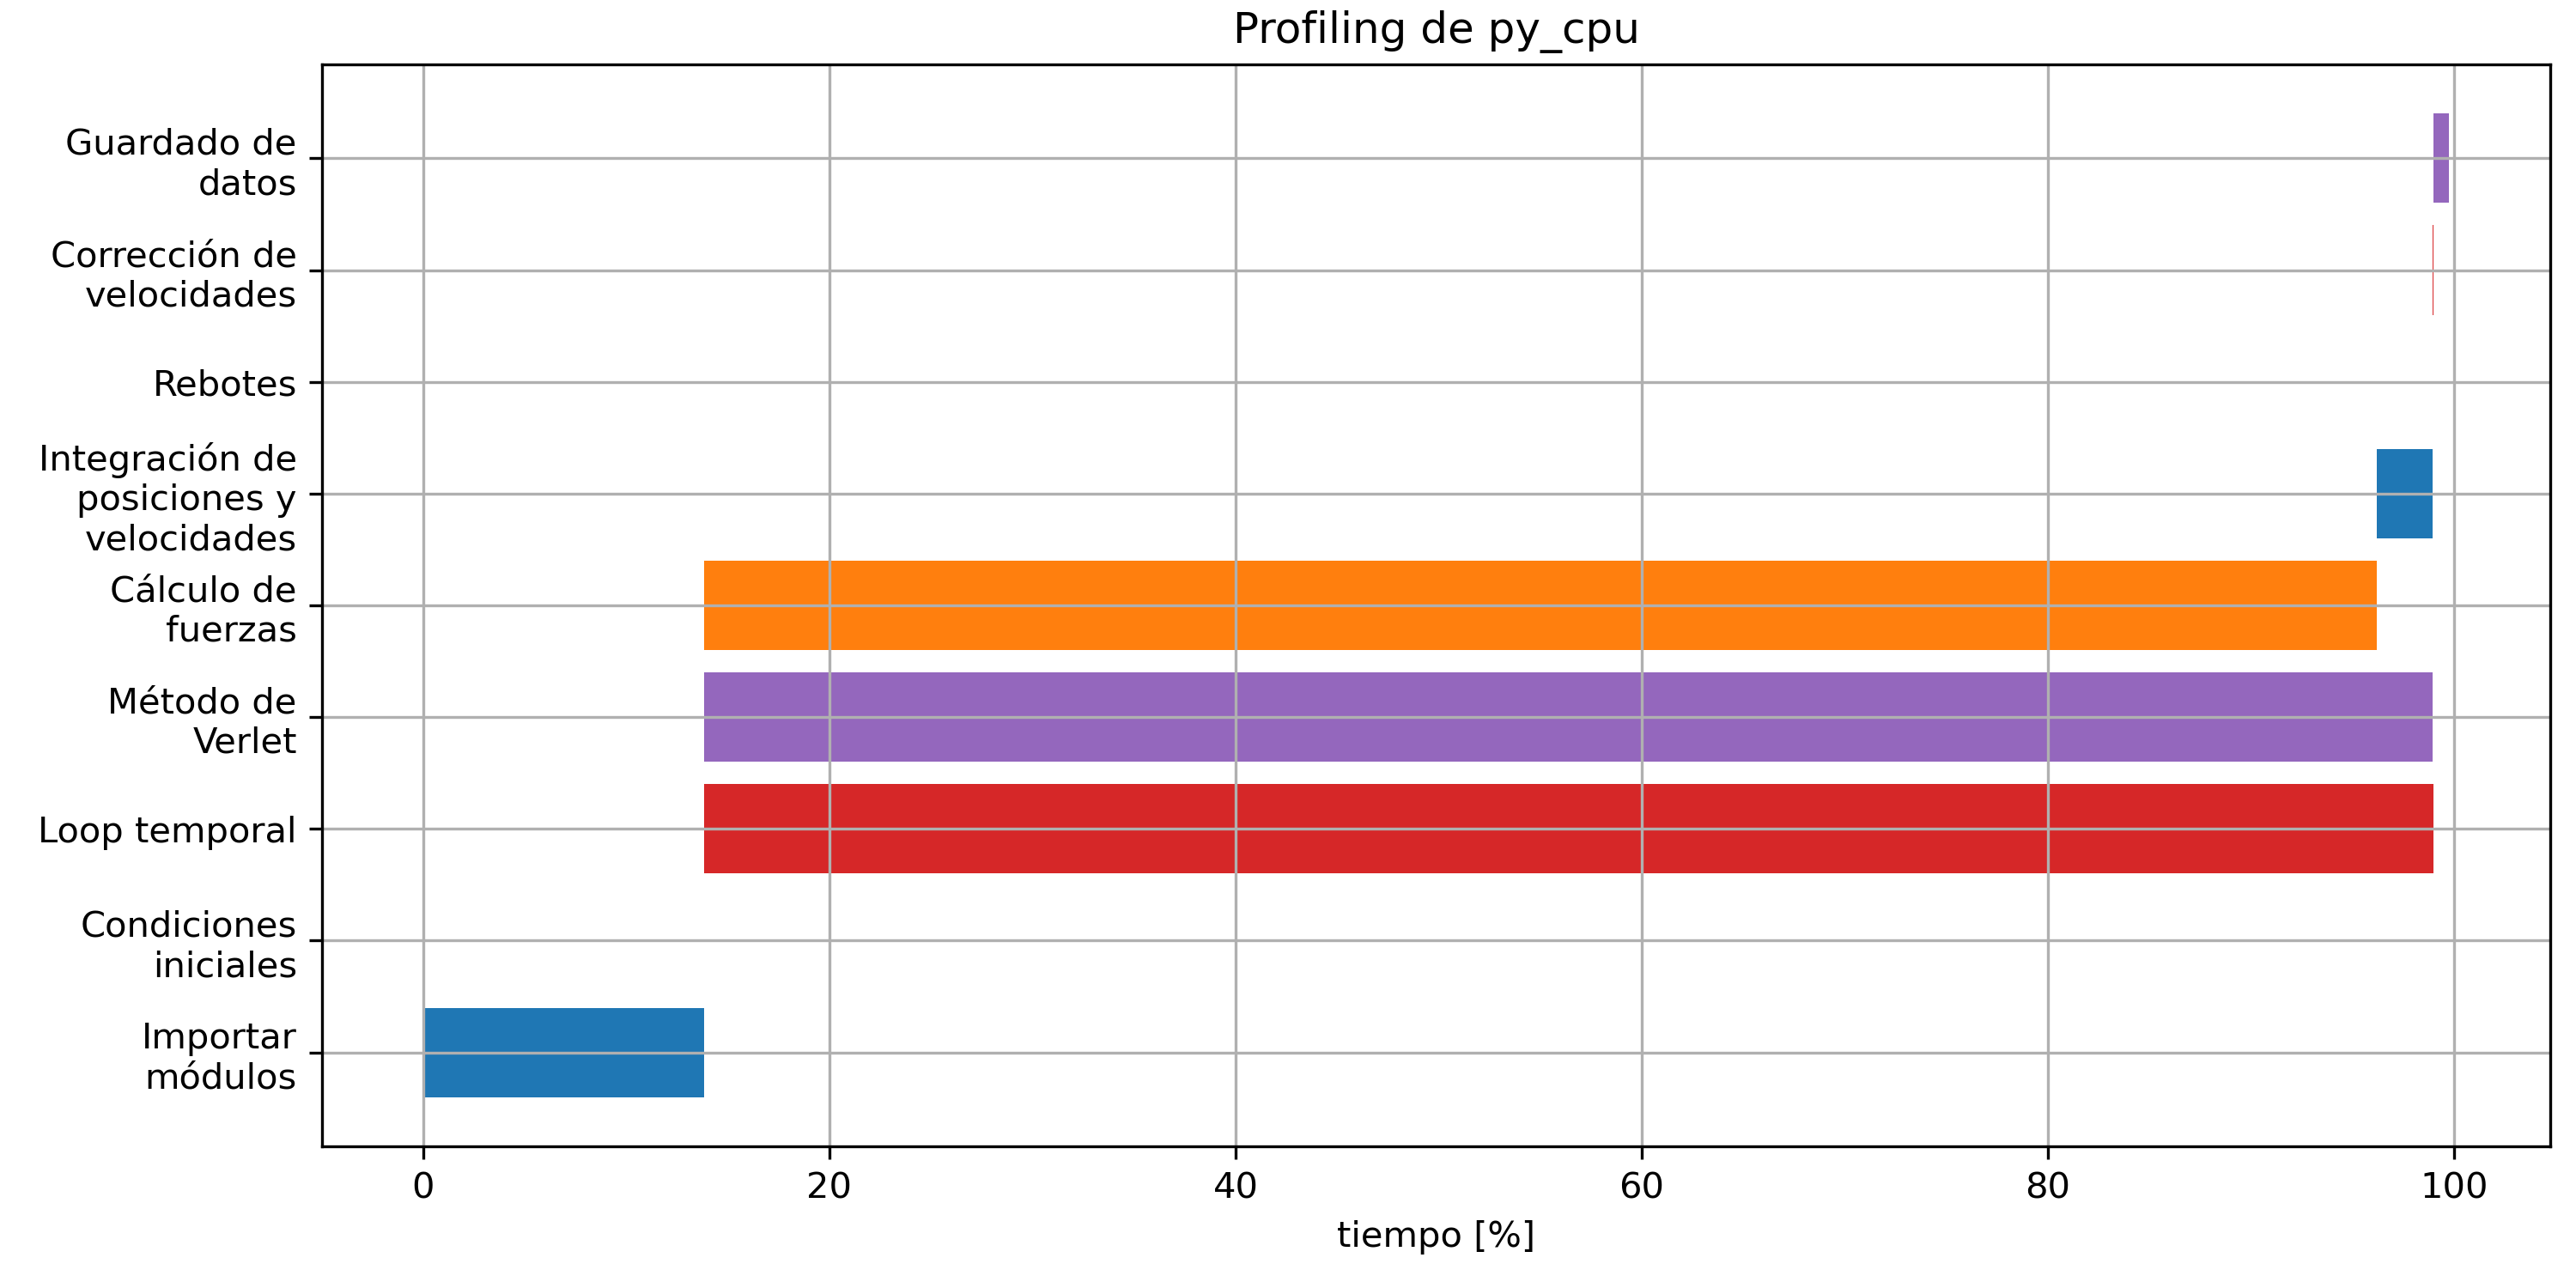
\includegraphics[clip=true,width=\columnwidth]{Profiling de py_cpu.png}
    \caption{}
     \label{fig:Profiling de py_cpu}
\end{figure}


\subsection{Versión 2: Python en paralelo}

\begin{itemize}
    \item Sólo intercambié numpy por cupy como para demostrar qué speed-up uno podría obtener con un código 
    \item \textcolor{blue}{Escribir ''import numpy as np'' $\rightarrow$ ''import cupy as np''}
    \item \textcolor{red}{Profiling. Ver qué CPU y GPU estoy usando} y análisis
\end{itemize}

\begin{figure}[h]
    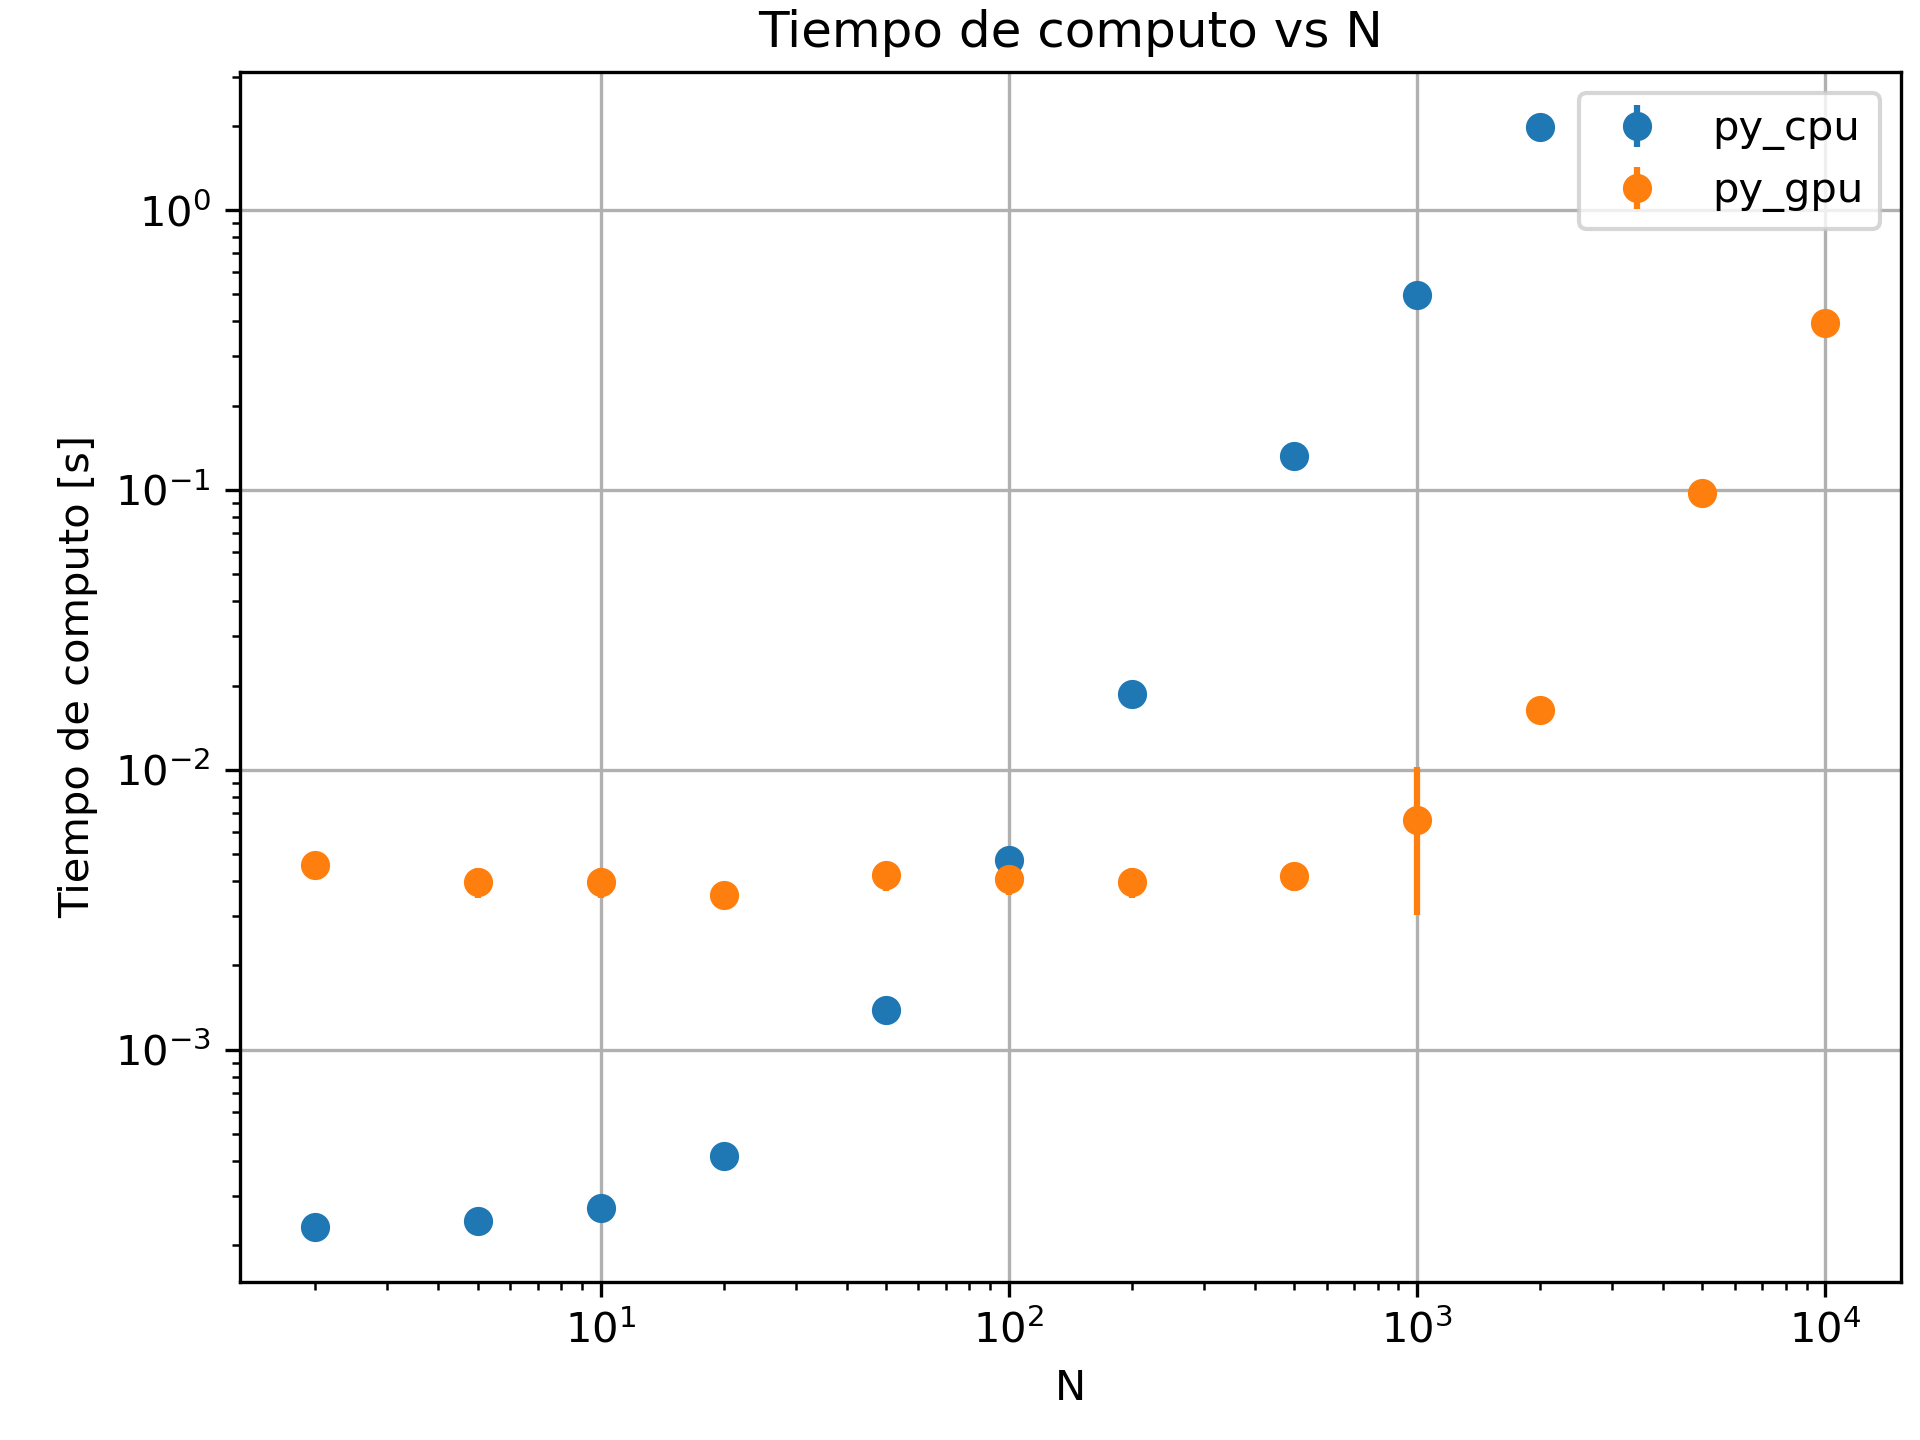
\includegraphics[clip=true,width=\columnwidth]{tiempo_de_computo_vs_N_py_all.png}
    \caption{Gráfico de tiempo de cómputo (py_cu y py_gpu)}
     \label{fig:tiempo_de_computo_vs_N_py_all}
\end{figure}

\begin{figure}[h]
    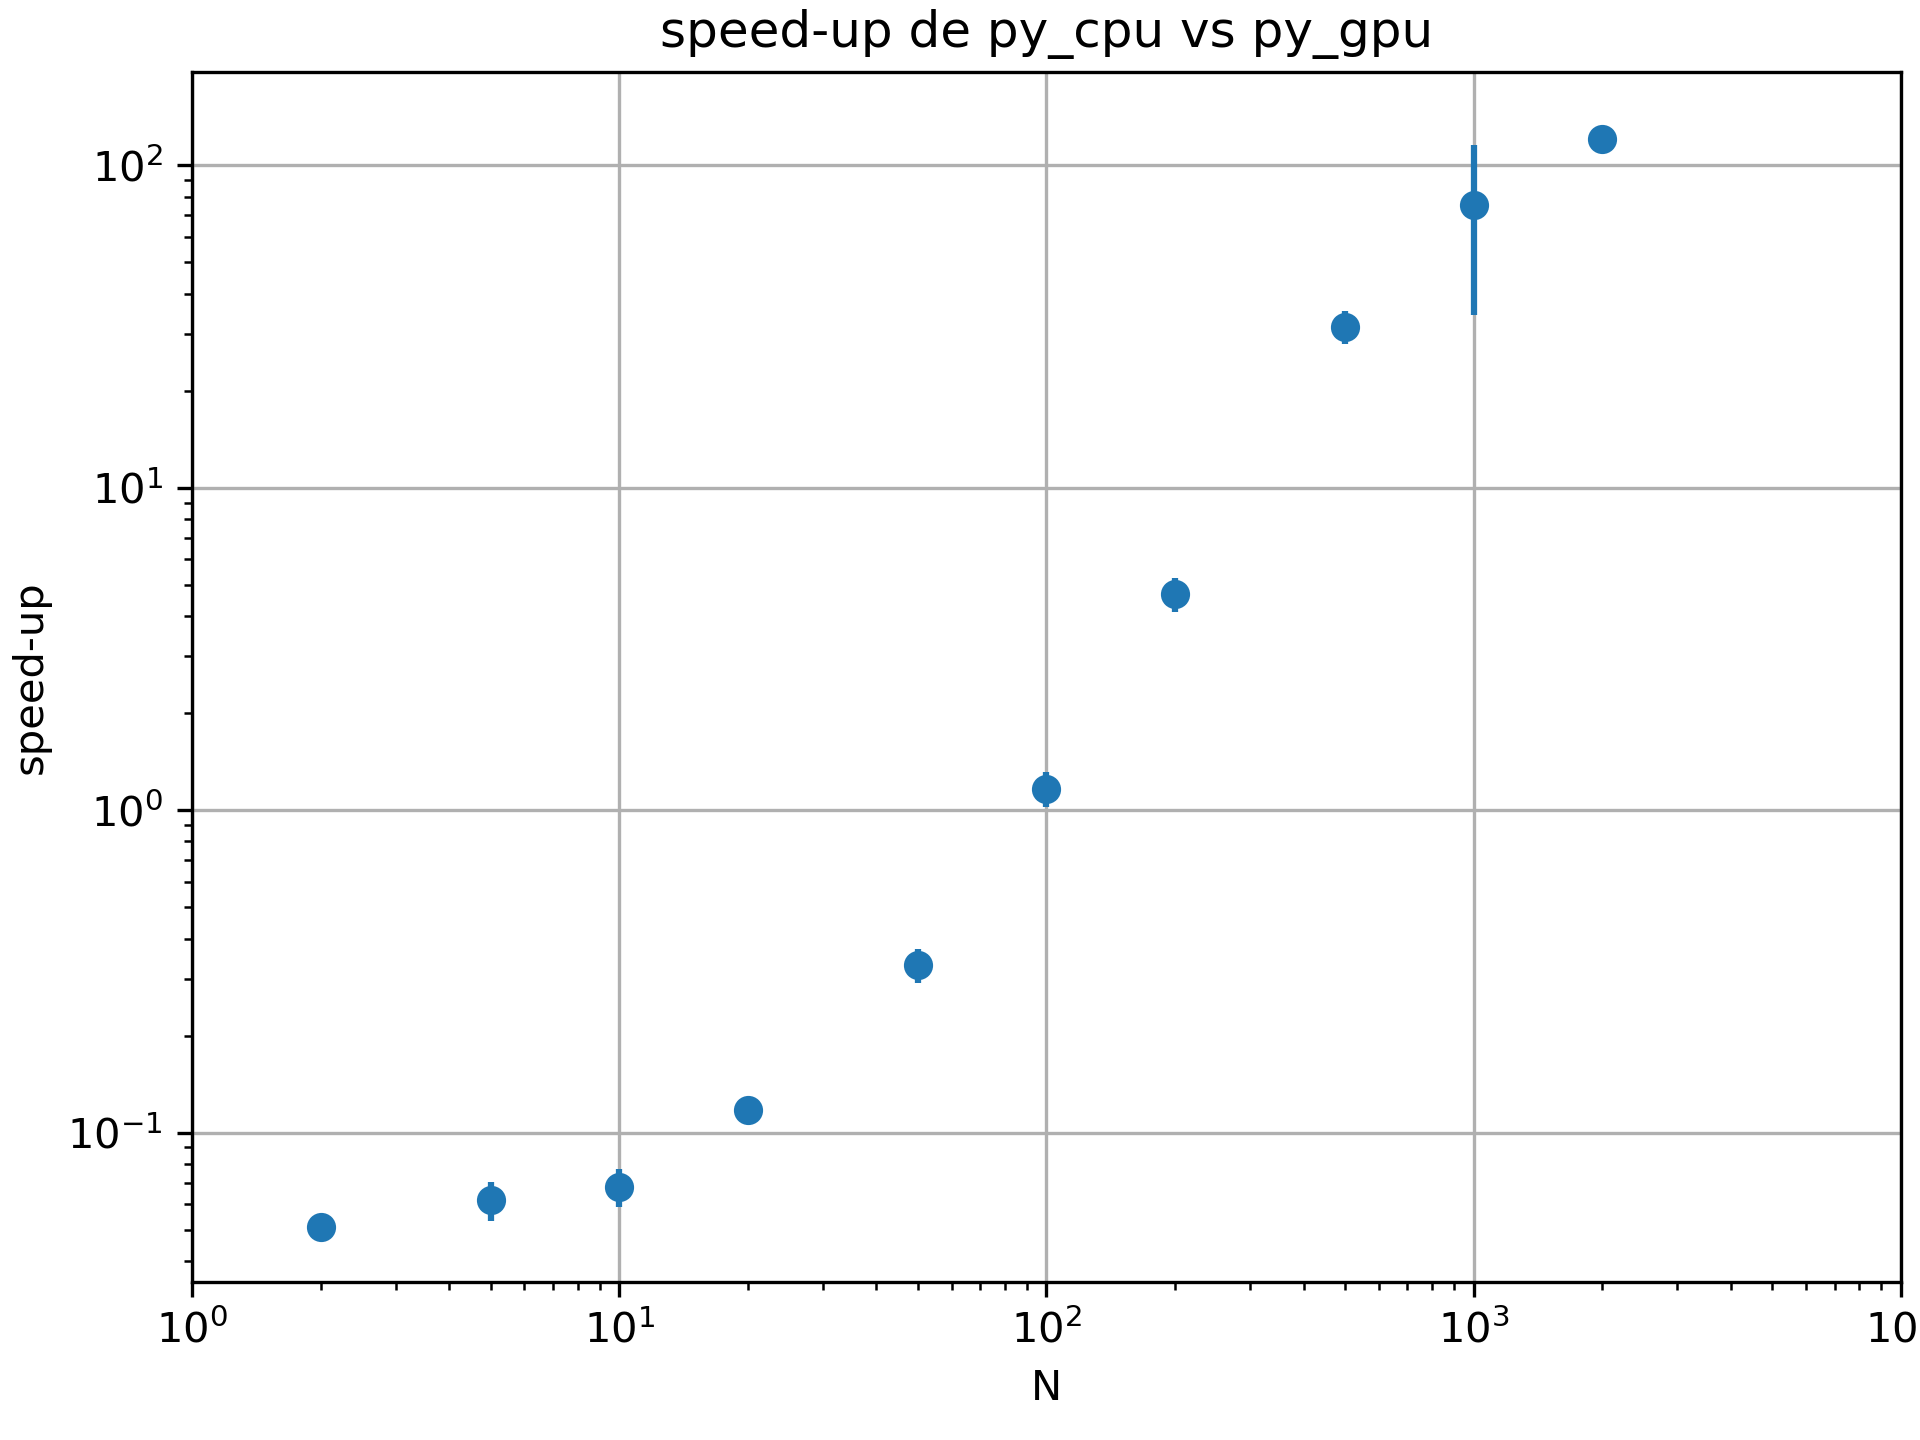
\includegraphics[clip=true,width=\columnwidth]{py_cpu_vs_py_gpu.png}
    \caption{Gráfico de speed-up respecto a py_cpu}
     \label{fig:py_cpu_vs_py_gpu}
\end{figure}

\begin{figure}[h]
    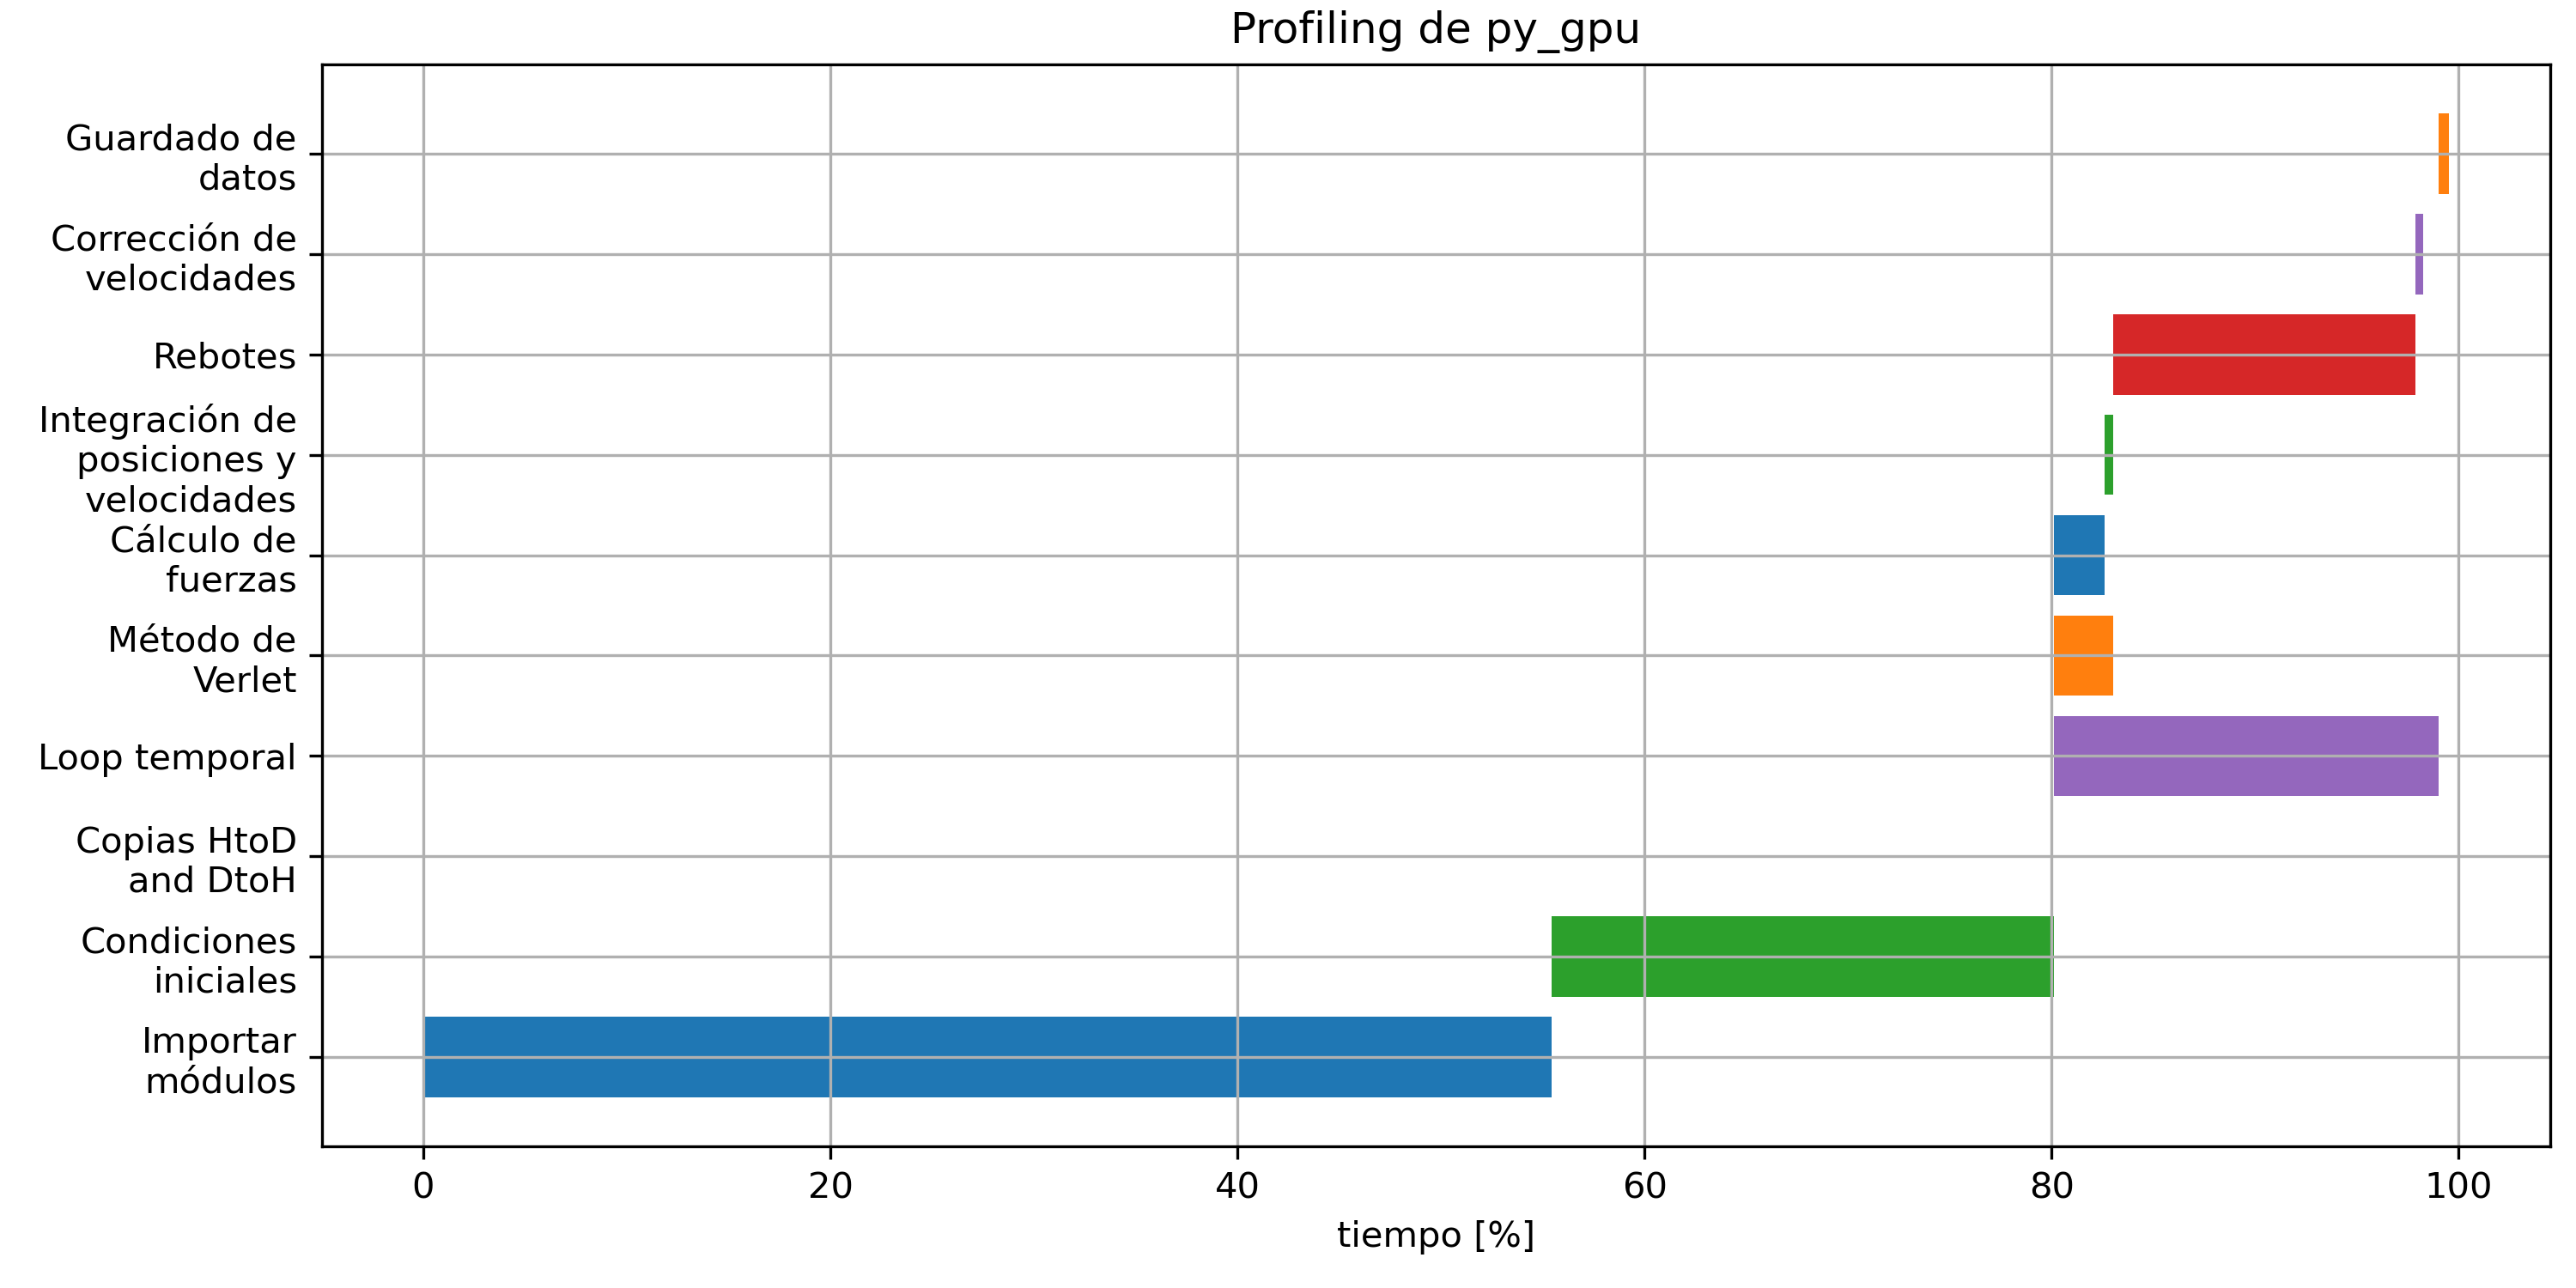
\includegraphics[clip=true,width=\columnwidth]{Profiling de py_gpu.png}
    \caption{}
     \label{fig:Profiling de py_gpu}
\end{figure}




\subsection{Versión 3: C++ en serie}

\begin{itemize}
    \item Usé los loops de C++ para todos los cálculos. Las fuerzas ya no se calculan mediante una matriz.
    \item \textcolor{blue}{Poner la función de fuerzas}
    \item \textcolor{red}{Ver qué CPU estoy usando} y análisis
\end{itemize}


\begin{figure}[h]
    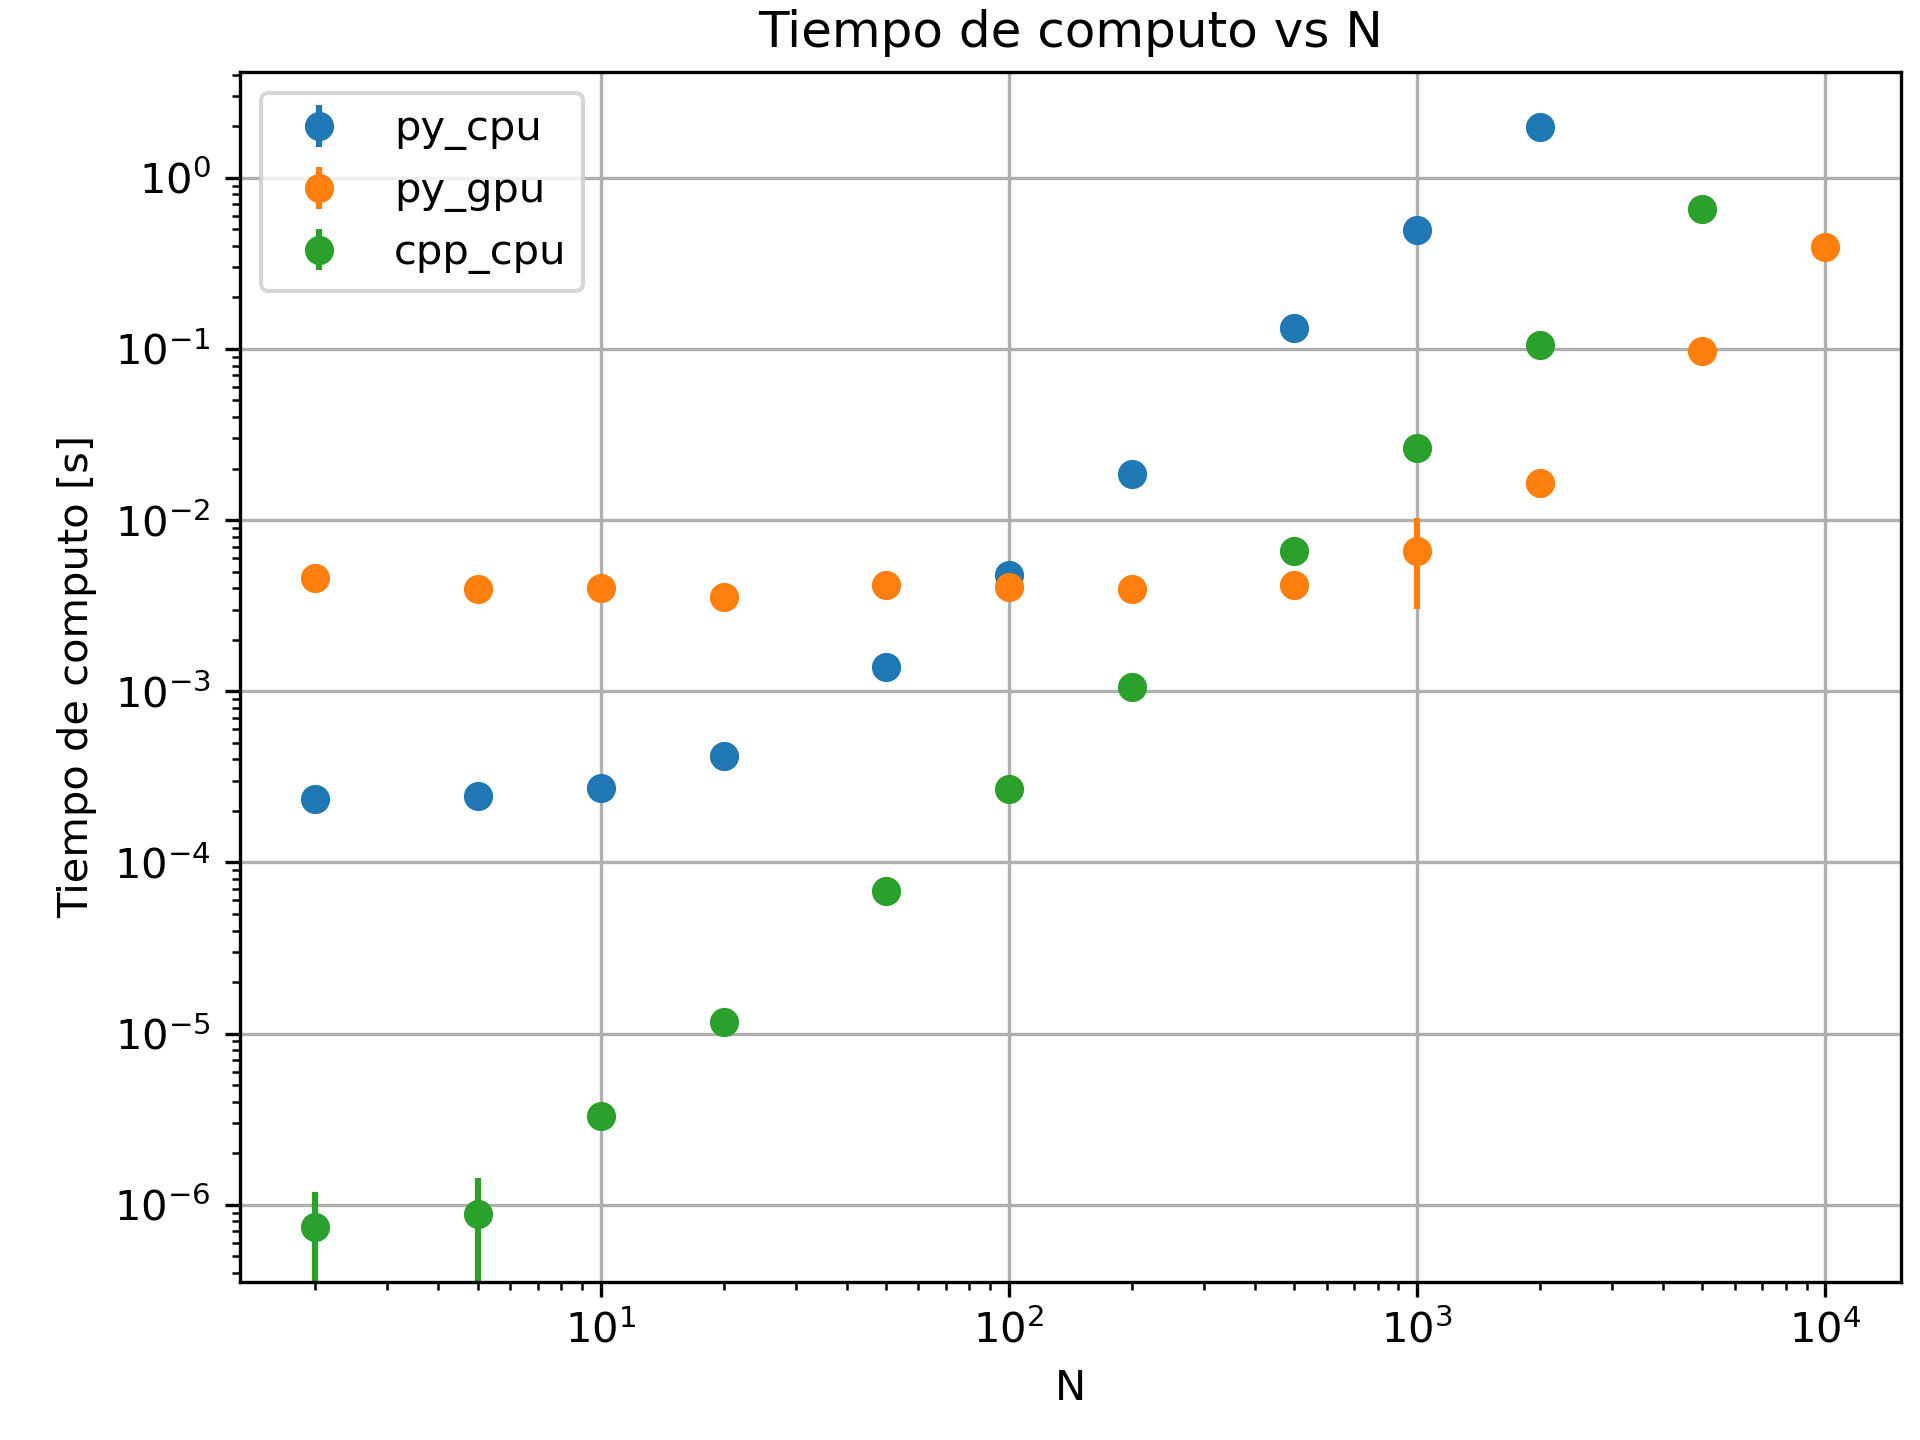
\includegraphics[clip=true,width=\columnwidth]{tiempo_de_computo_vs_N_py_all_and_cpp_cpu.png}
    \caption{Gráfico de tiempo de cómputo (py_cu, py_gpu y cpp_cpu)}
     \label{fig:tiempo_de_computo_vs_N_py_all_and_cpp_cpu}
\end{figure}


\begin{figure}[h]
    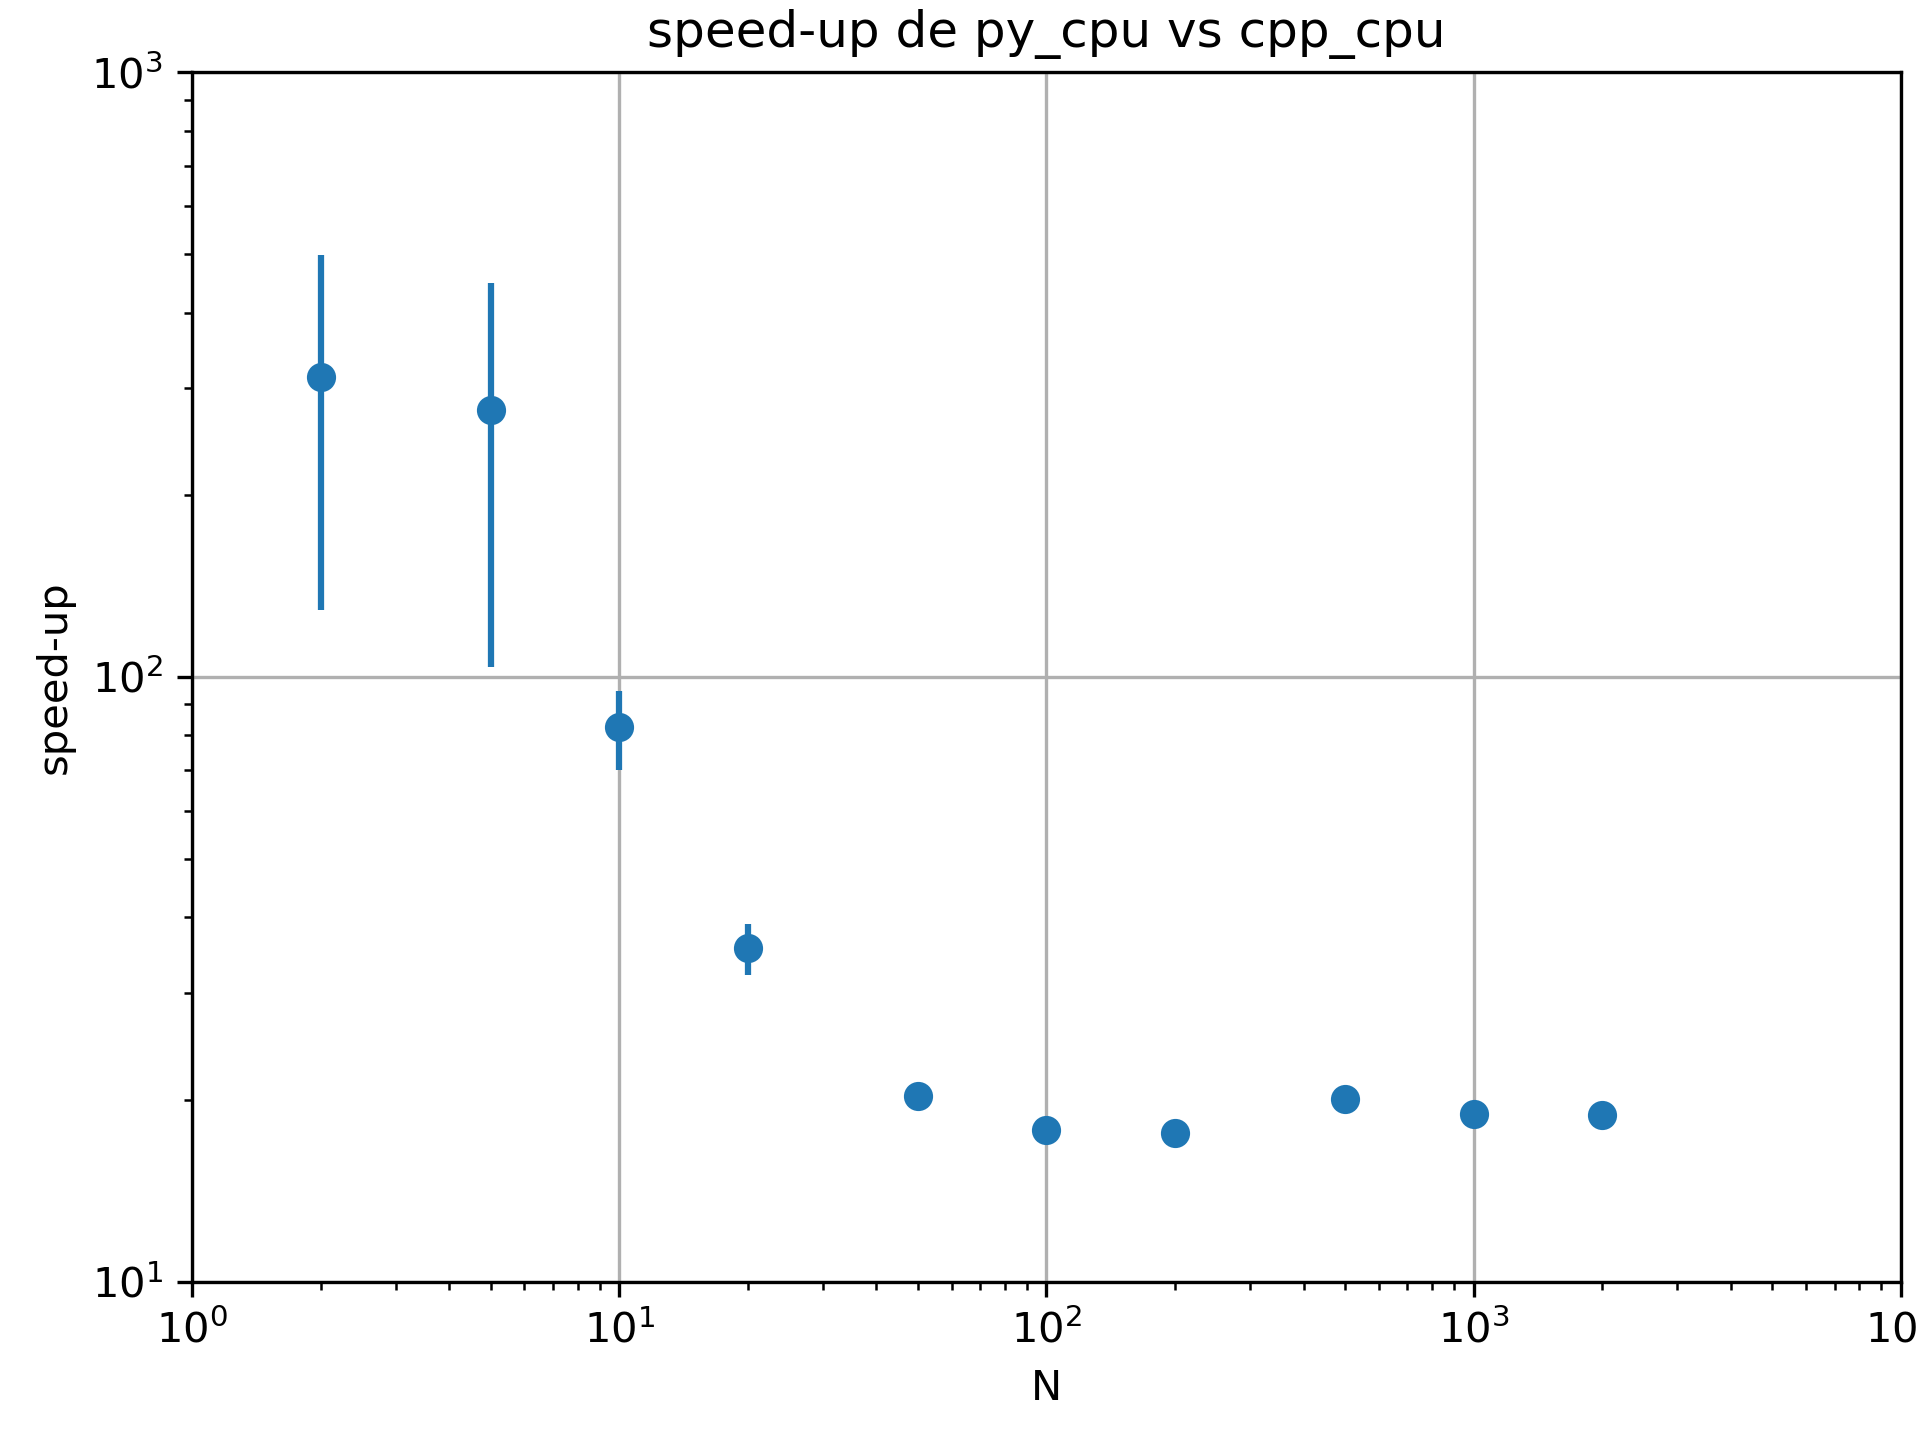
\includegraphics[clip=true,width=\columnwidth]{py_cpu_vs_cpp_cpu.png}
    \caption{Gráfico de speed-up respecto a py_cpu}
     \label{fig:py_cpu_vs_cpp_cpu}
\end{figure}

\begin{figure}[h]
    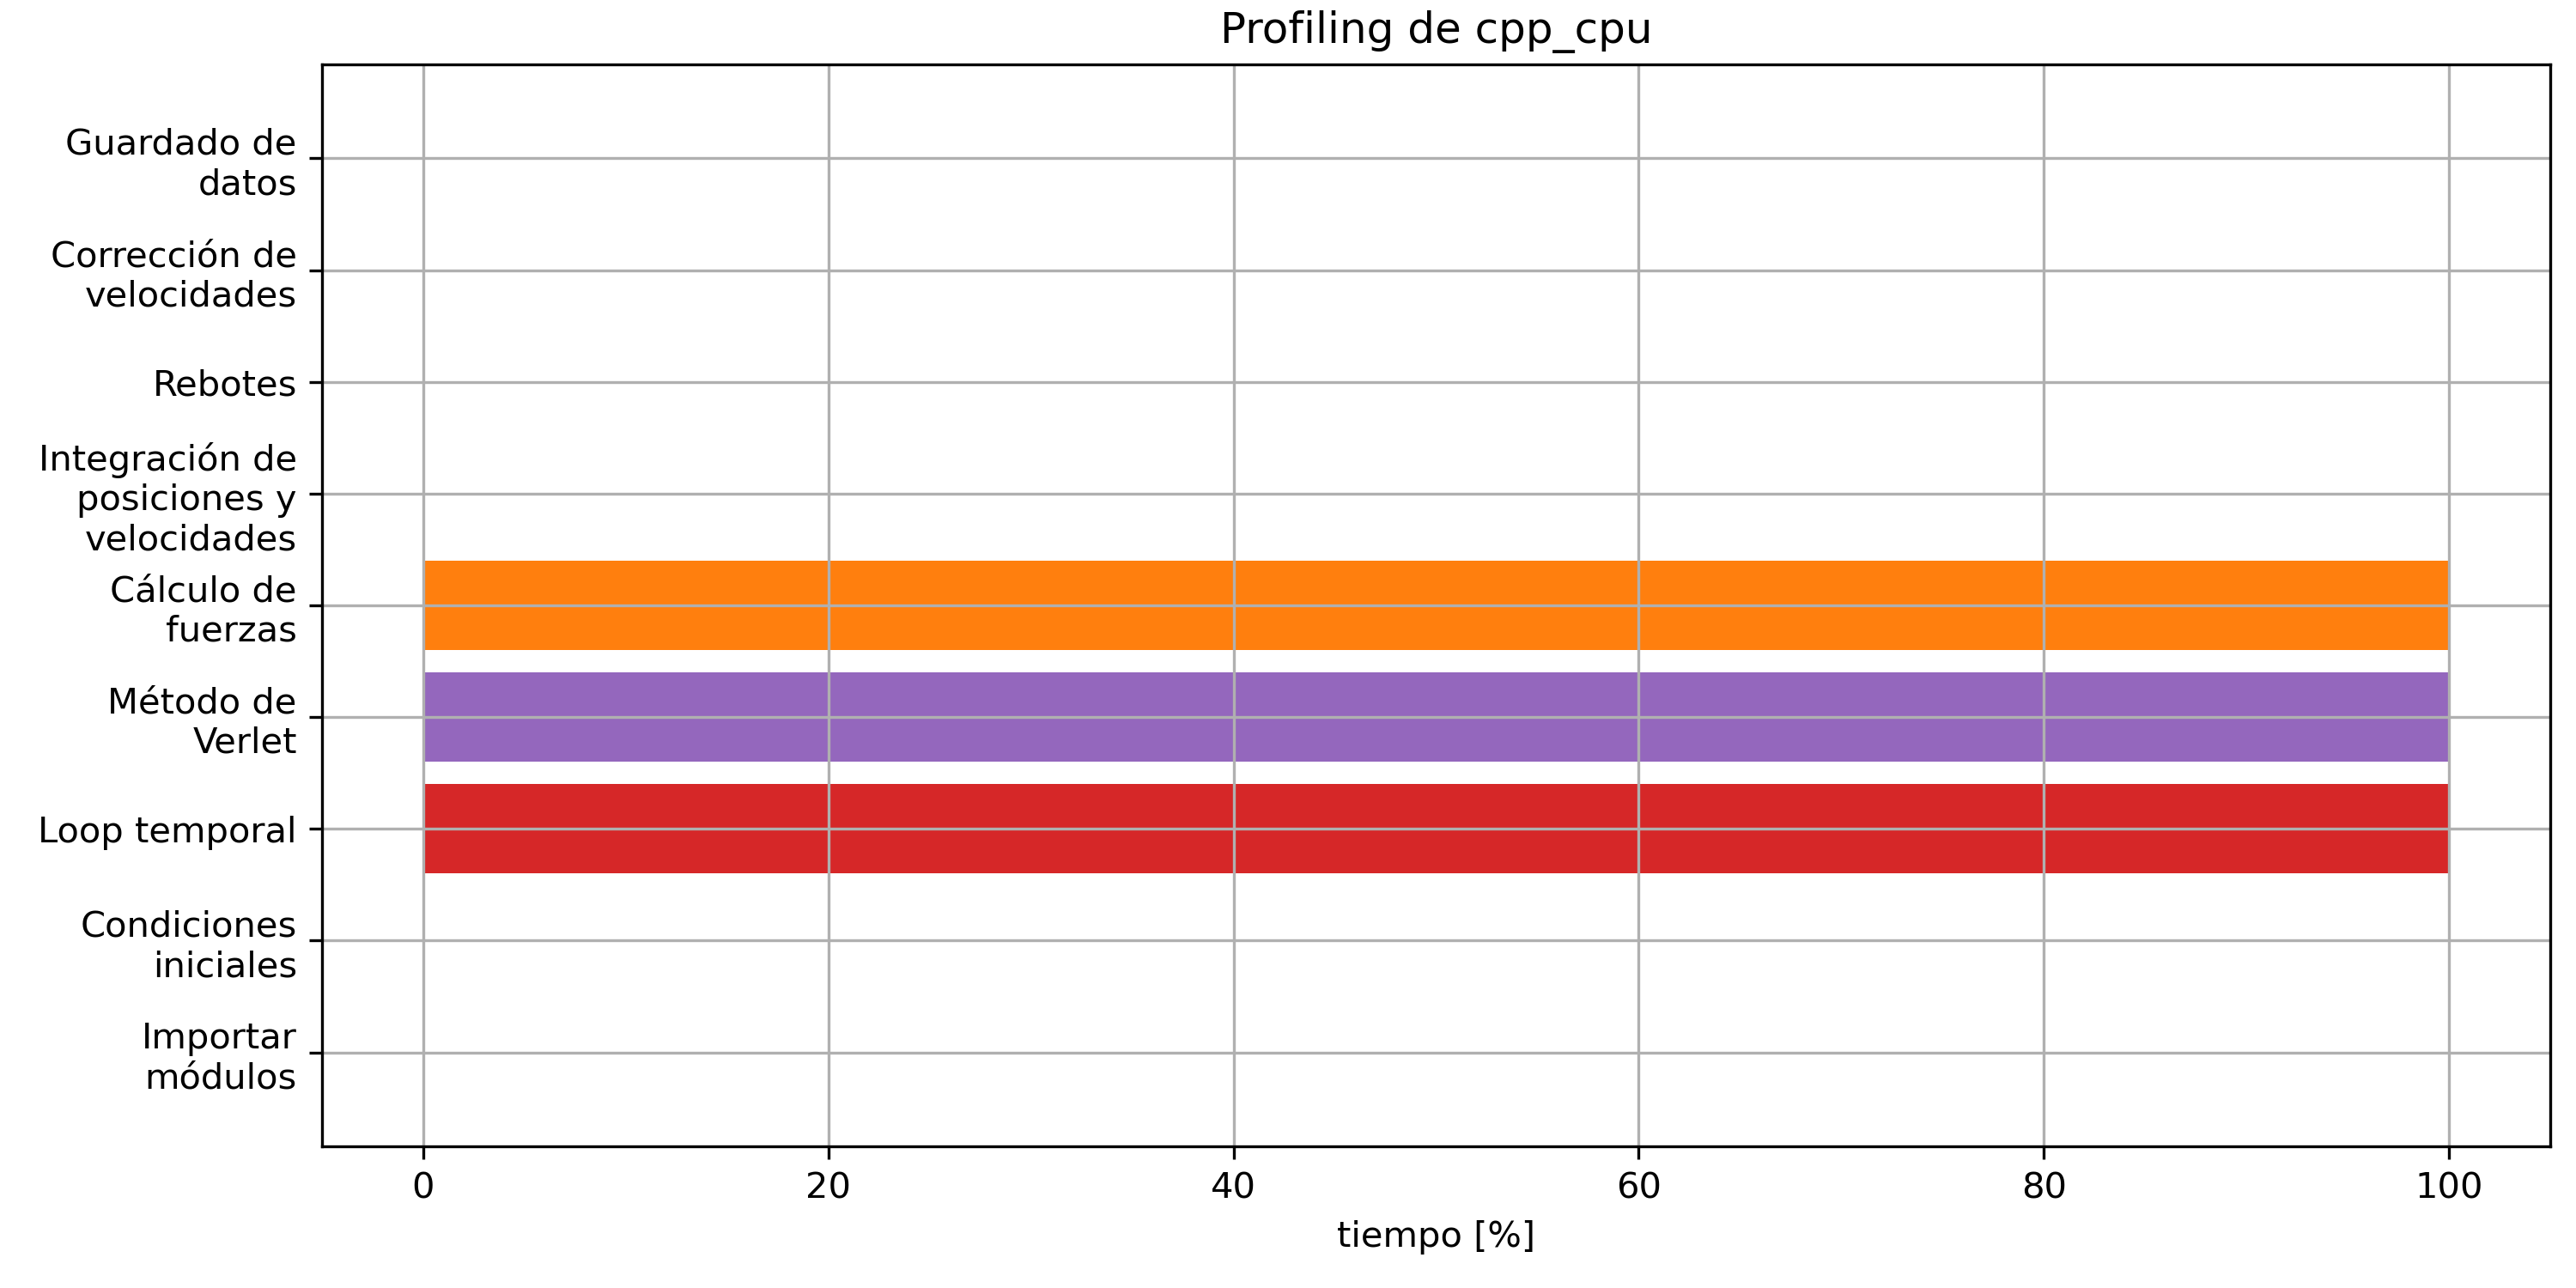
\includegraphics[clip=true,width=\columnwidth]{Profiling de cpp_cpu.png}
    \caption{}
     \label{fig:Profiling de cpp_cpu}
\end{figure}


\subsection{Versión 4: C++ en paralelo v1}

\begin{itemize}
    \item Usé kernels para hacer cada una de las cuentas, un blocksize de \textcolor{red}{256?} y solo hice copias al inicio y al final de la evolución
    \item \textcolor{blue}{Volver a poner los items al inicio de "implementación" y poner al lado de cada item una flecha y la declaración de los kernels}
    \item \textcolor{blue}{}
    \item \textcolor{blue}{}
    \item \textcolor{red}{. Ver qué CPU y GPU estoy usando} y análisis
\end{itemize}

\begin{figure}[h]
    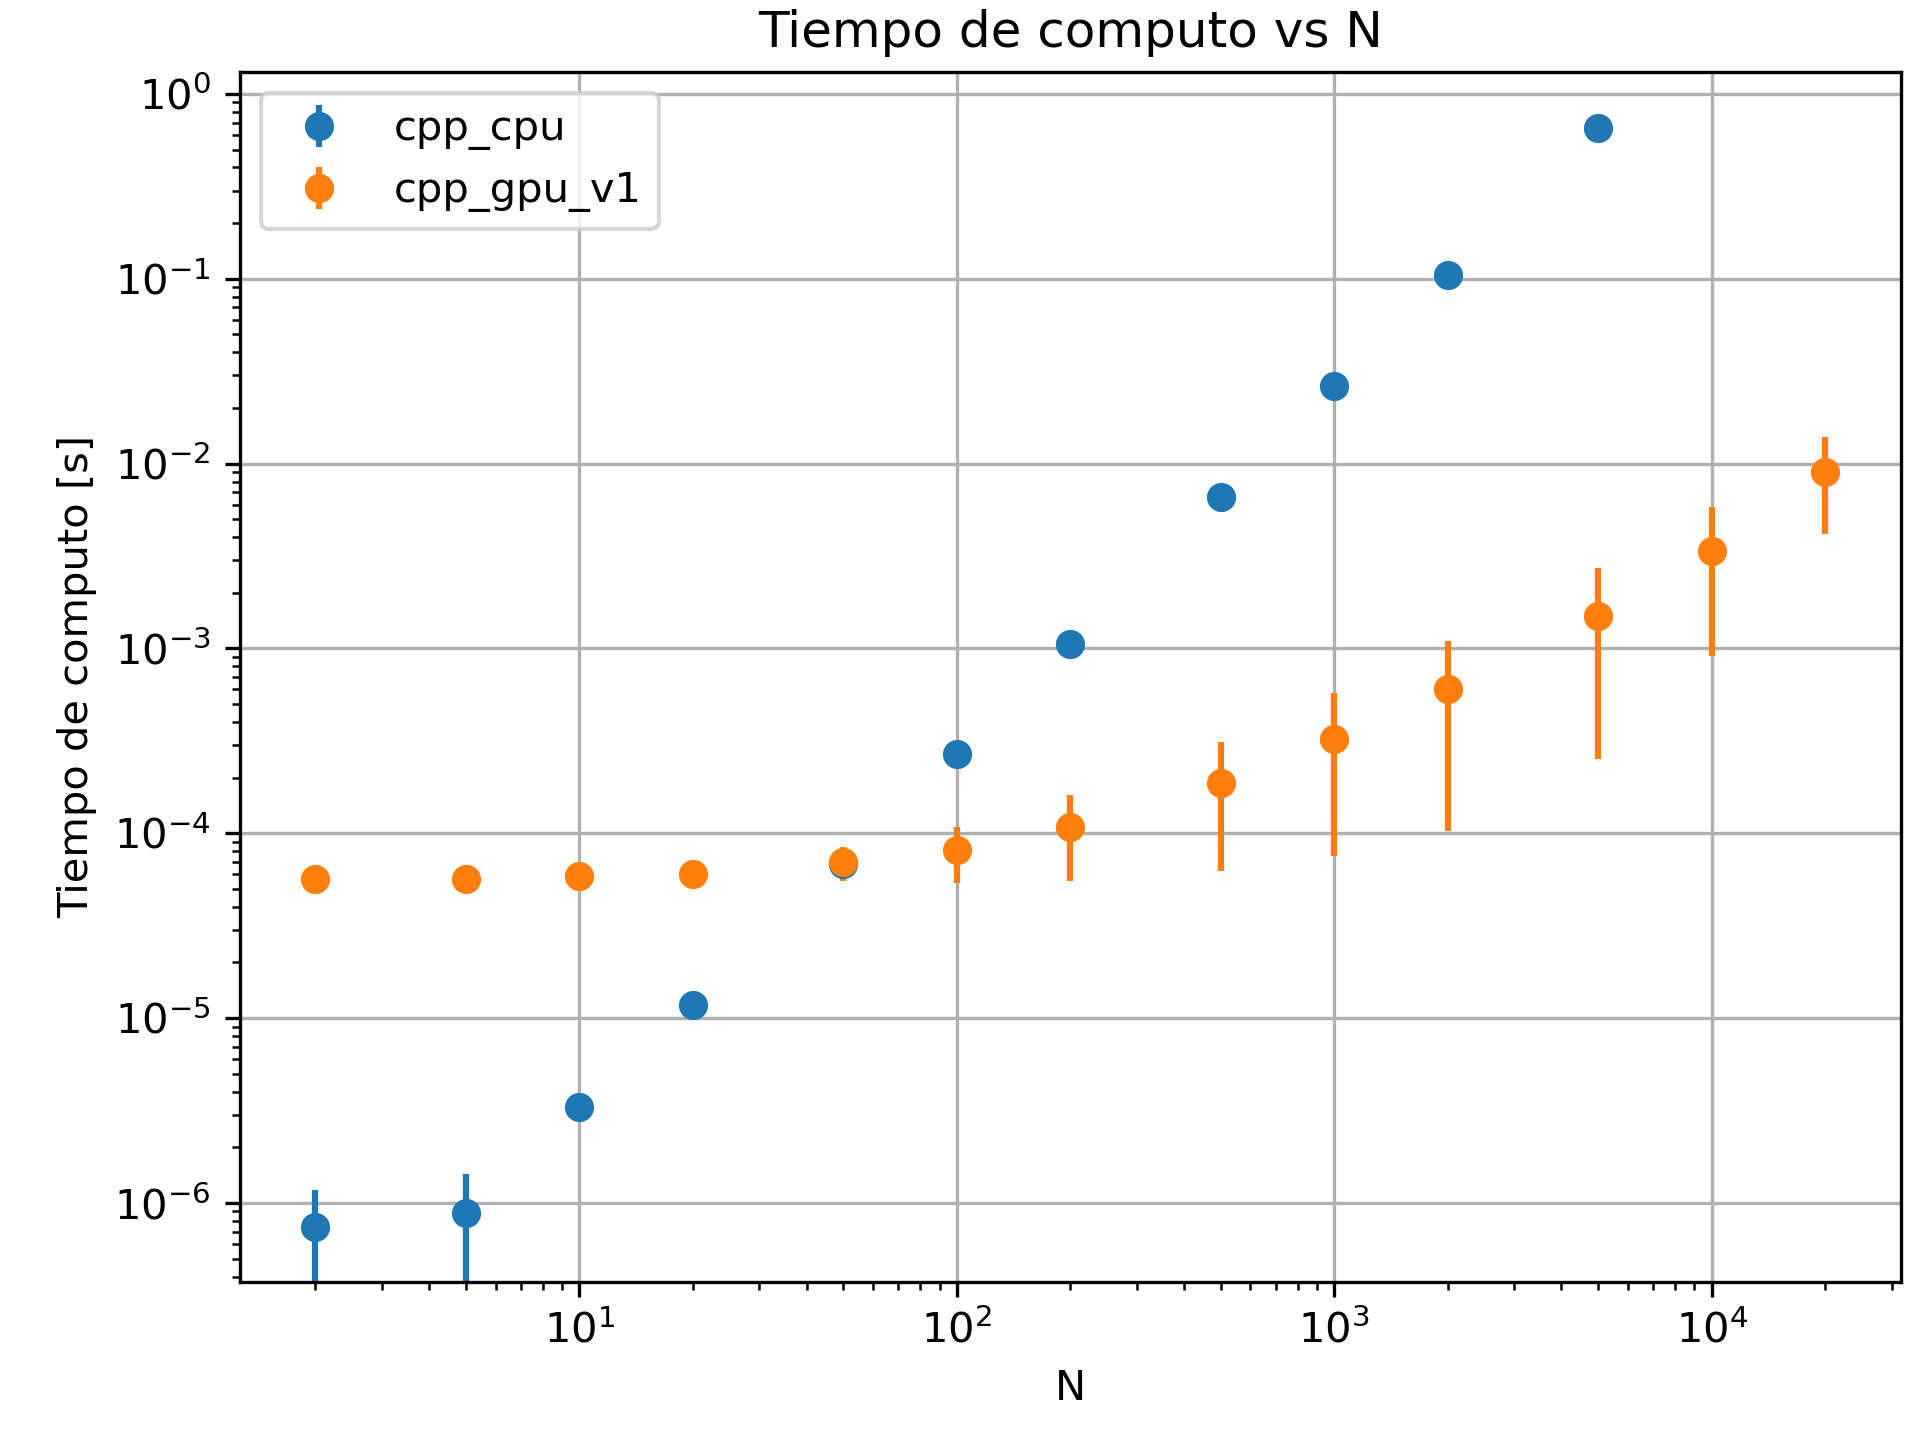
\includegraphics[clip=true,width=\columnwidth]{tiempo_de_computo_vs_N_cpp_cpu_and_gpu_v1.png}
    \caption{Gráfico de tiempo de cómputo (cpp_cpu, cpp_gpu_v1)}
     \label{fig:tiempo_de_computo_vs_N_cpp_cpu_and_gpu_v1}
\end{figure}


\begin{figure}[h]
    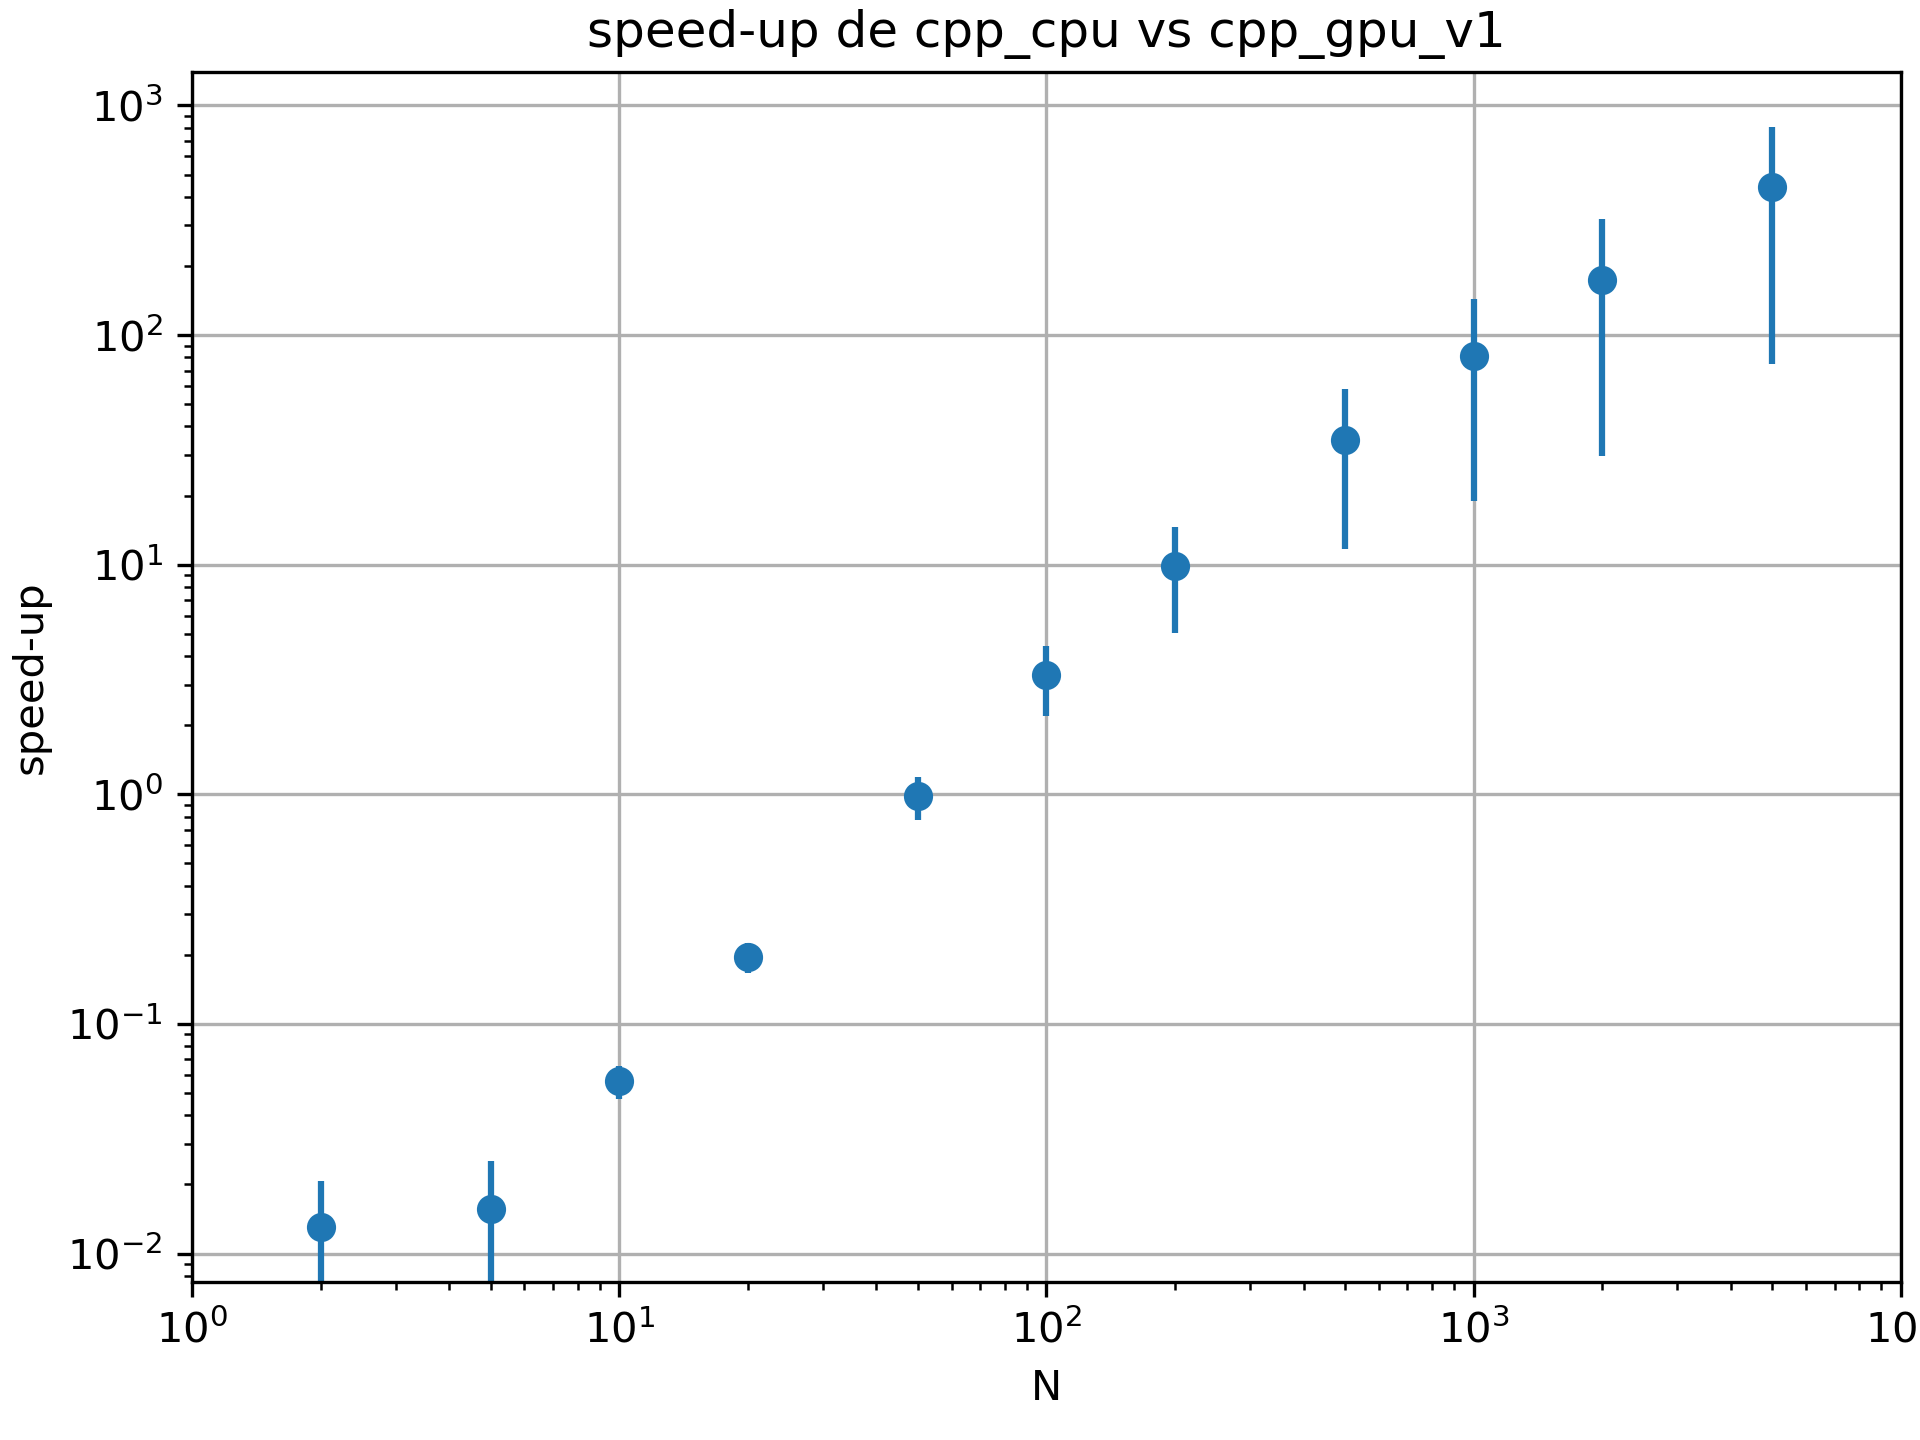
\includegraphics[clip=true,width=\columnwidth]{cpp_cpu_vs_cpp_gpu_v1.png}
    \caption{Gráfico de speed-up respecto a cpp_cpu}
     \label{fig:cpp_cpu_vs_cpp_gpu_v1}
\end{figure}


\begin{figure}[h]
    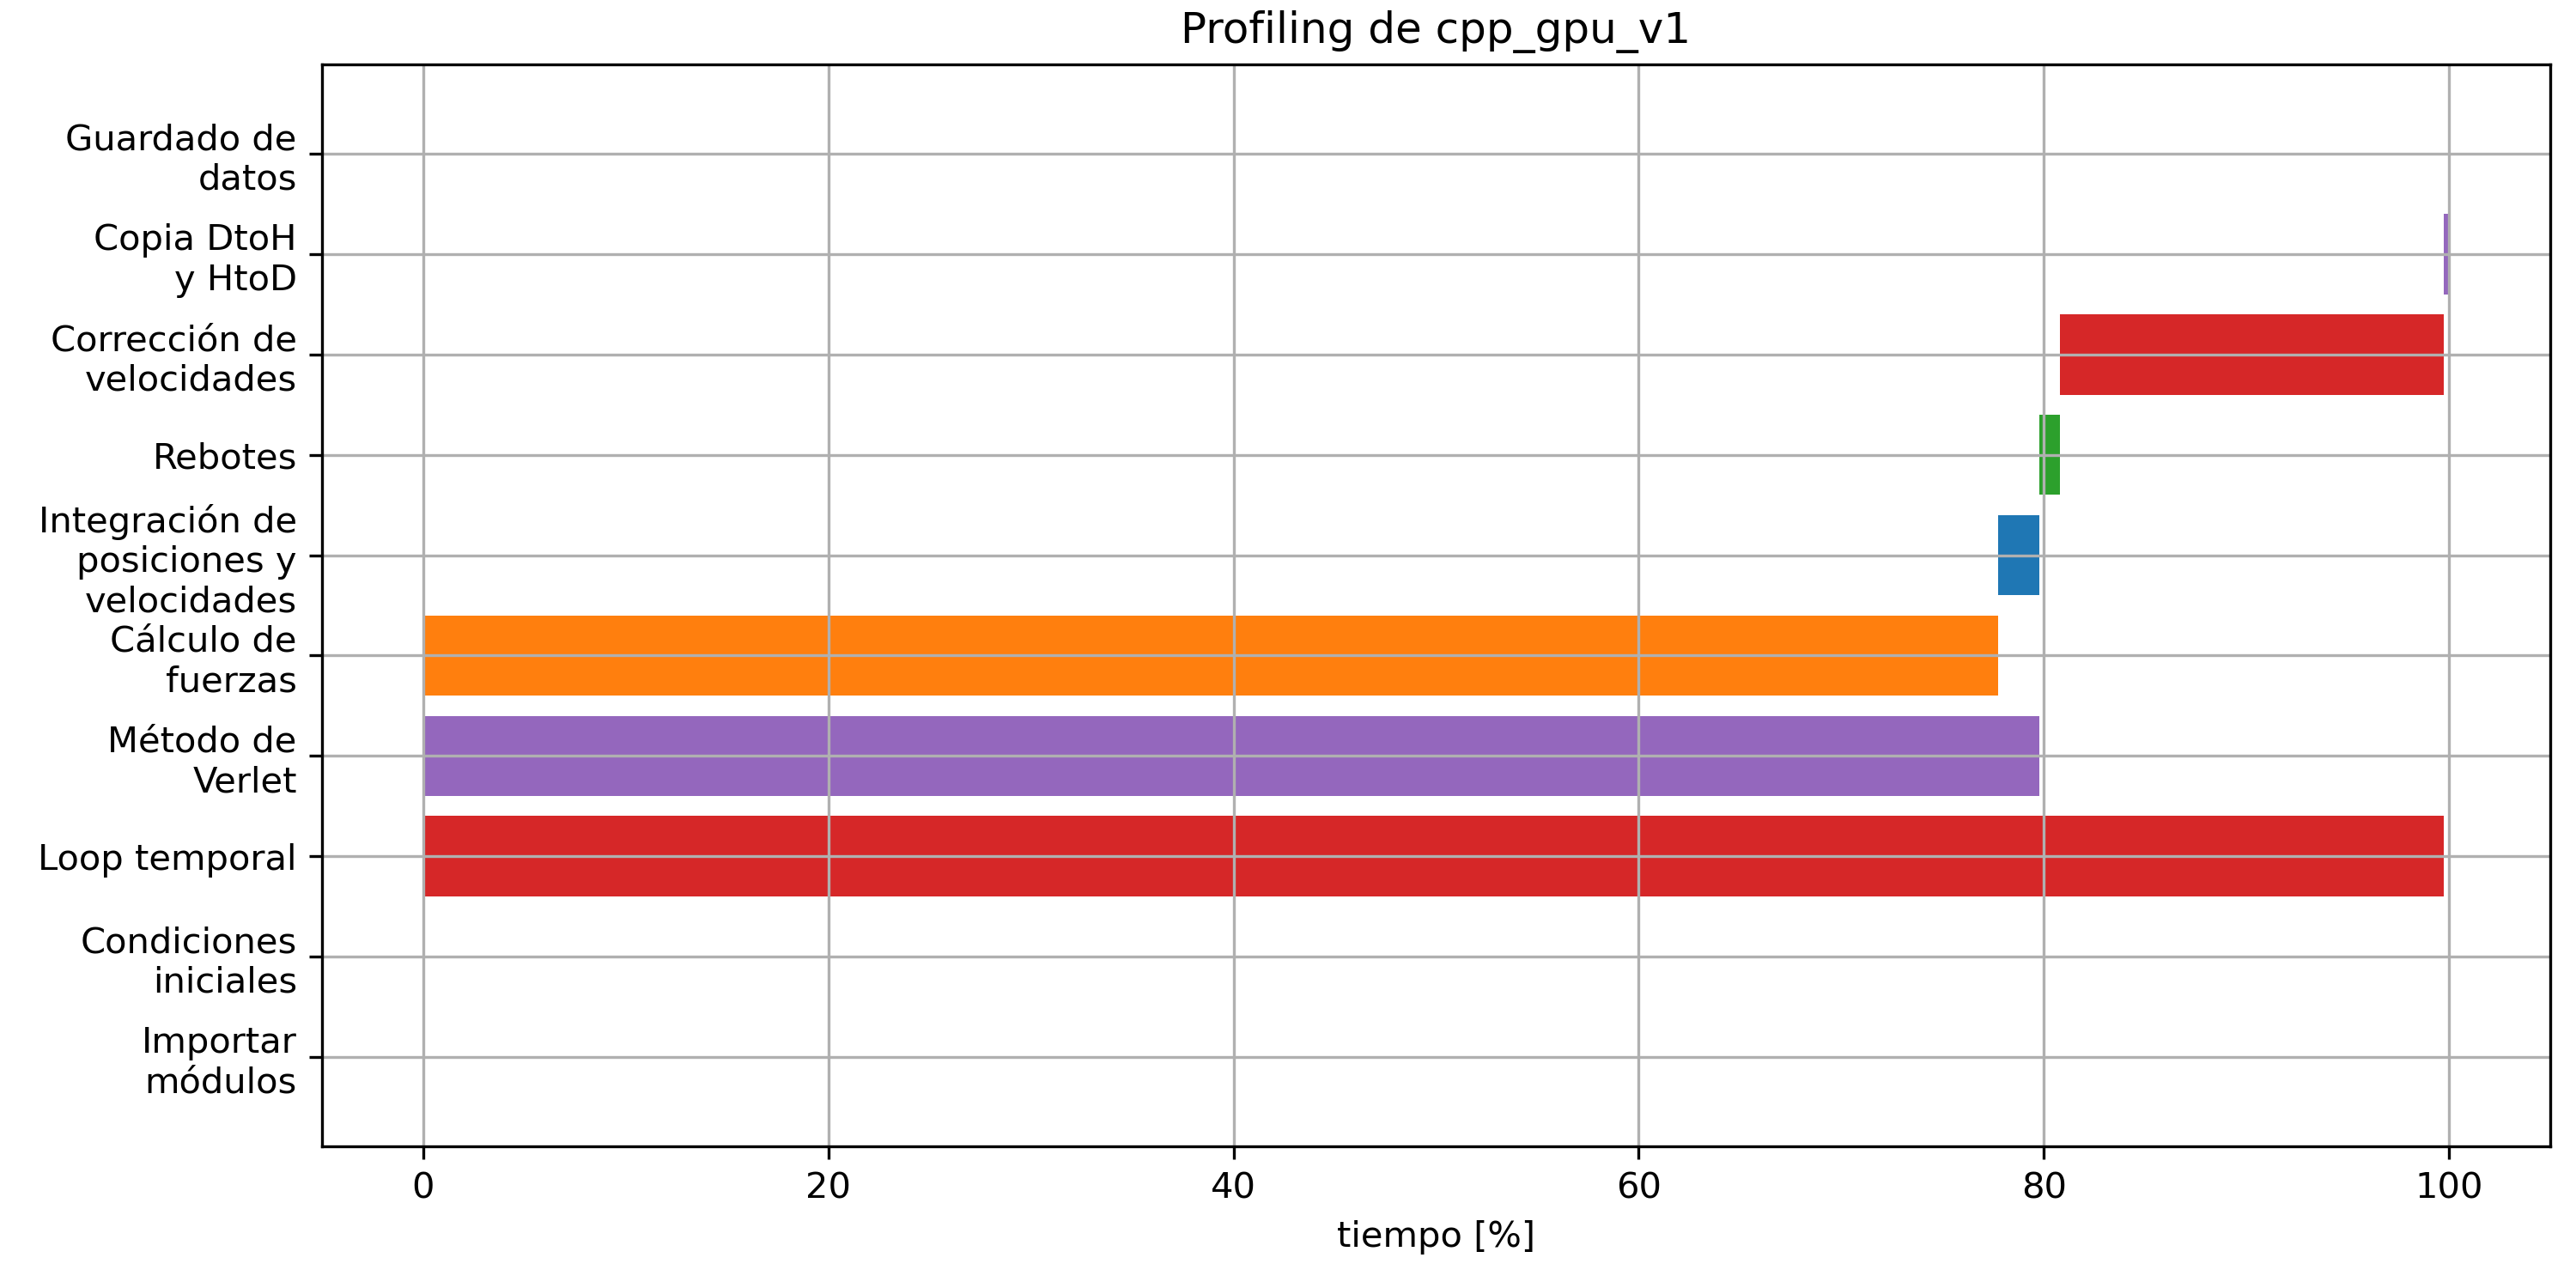
\includegraphics[clip=true,width=\columnwidth]{Profiling de cpp_gpu_v1.png}
    \caption{Profiling}
     \label{fig:Profiling de cpp_gpu_v1}
\end{figure}




\subsection{Versión 5: C++ en paralelo v2}

\begin{itemize}
    \item usé shared-memory
    \item \textcolor{blue}{Poner la sección en la que usé shared memory}
    \item \textcolor{red}{. Ver qué CPU y GPU estoy usando} y análisis
\end{itemize}

\begin{figure}[h]
    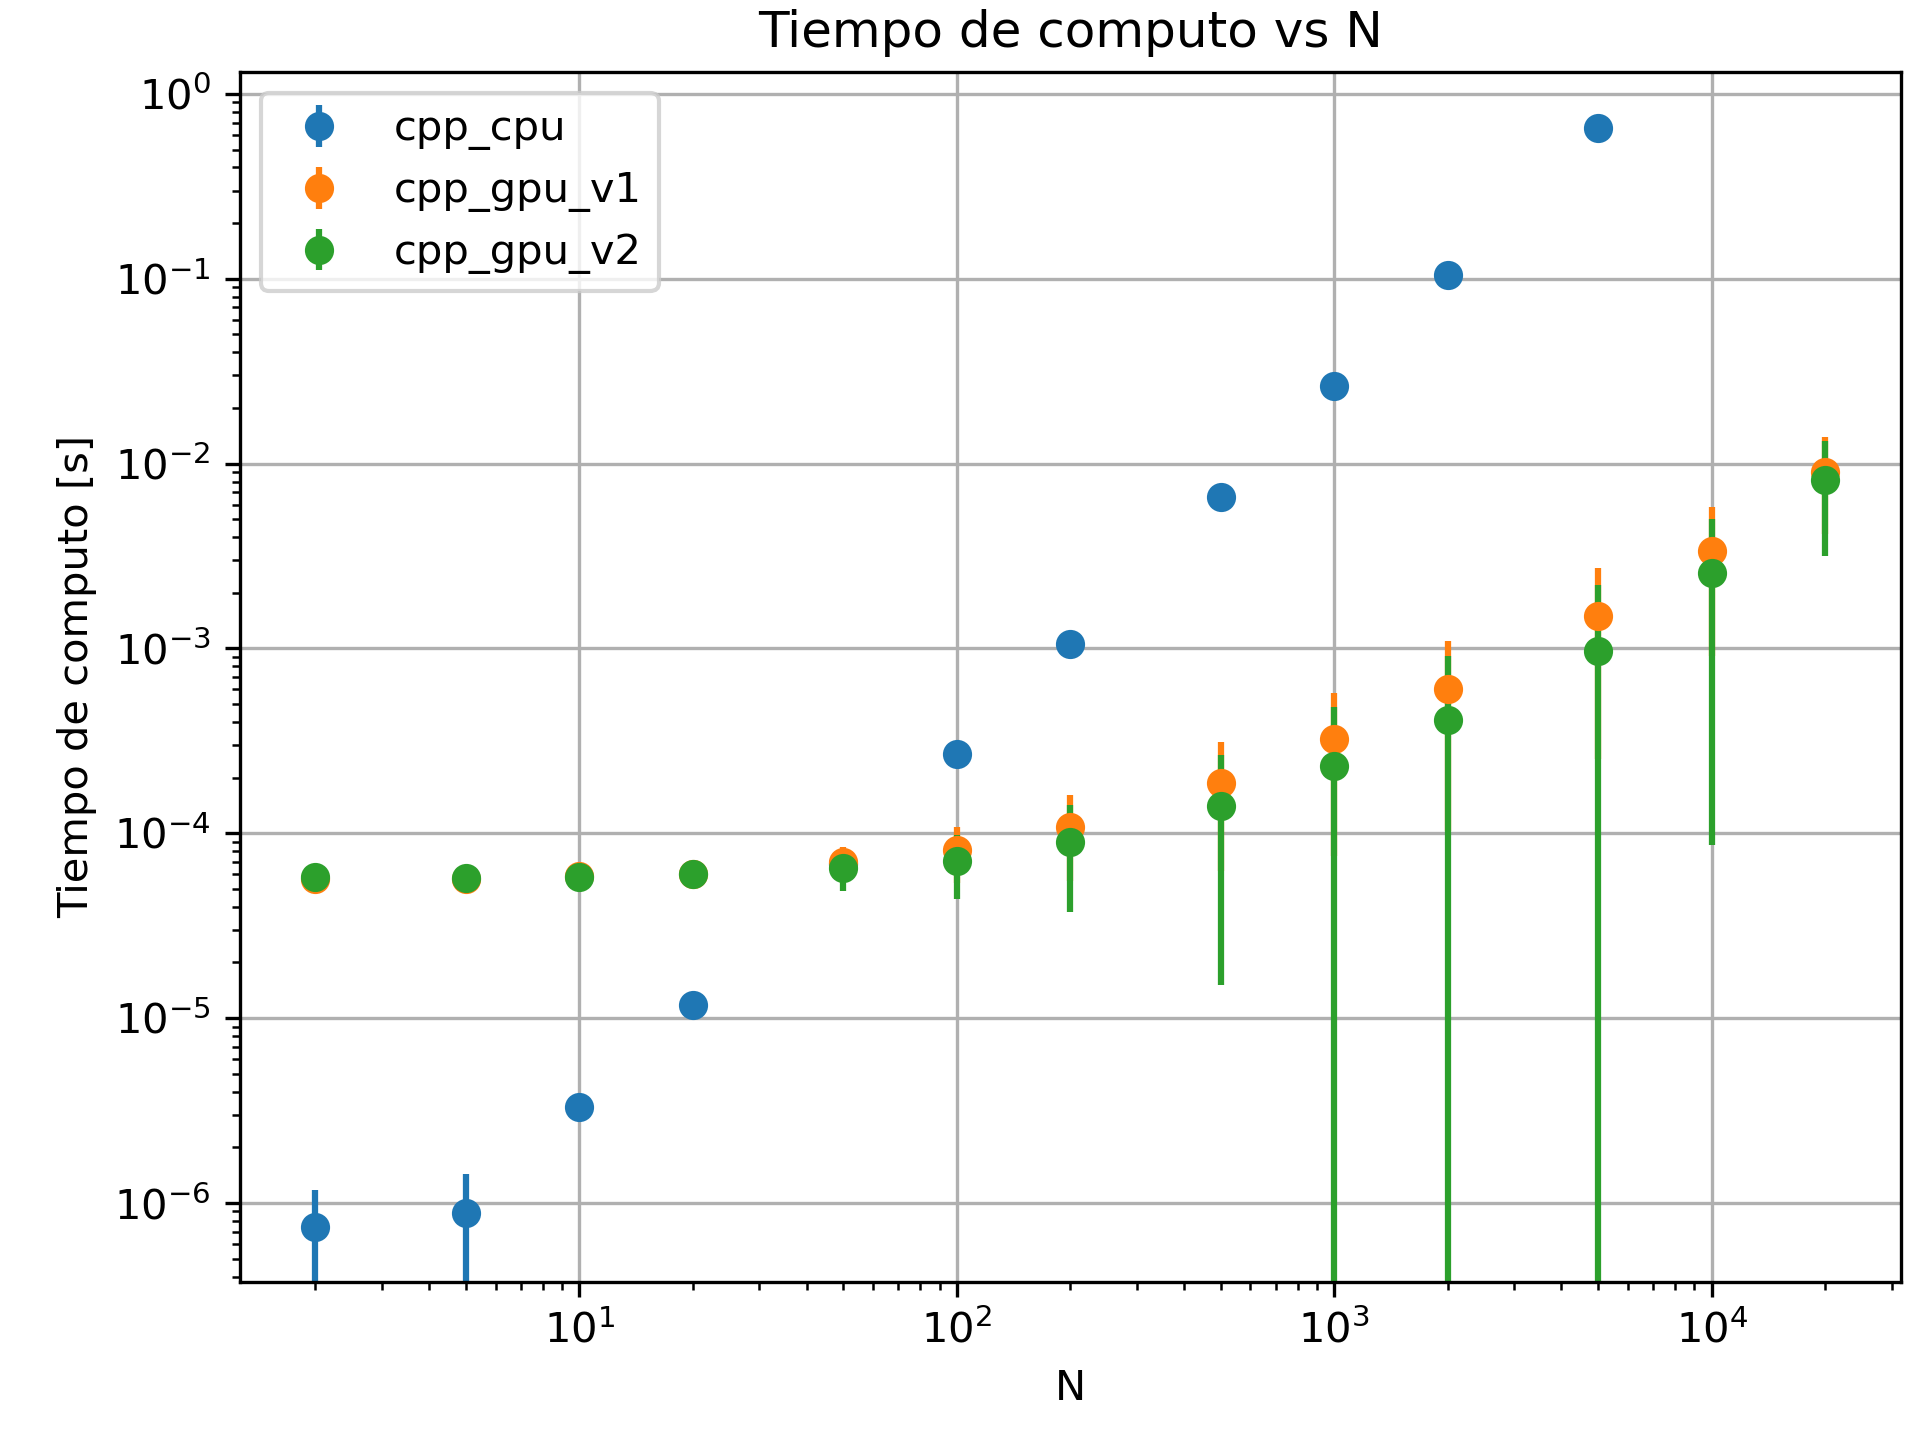
\includegraphics[clip=true,width=\columnwidth]{tiempo_de_computo_vs_N_cpp_all.png}
    \caption{Gráfico de tiempo de cómputo (cpp_cu, cpp_gpu_v1 y cpp_gpu_v2)}
     \label{fig:tiempo_de_computo_vs_N_cpp_all}
\end{figure}

\begin{figure}[h]
    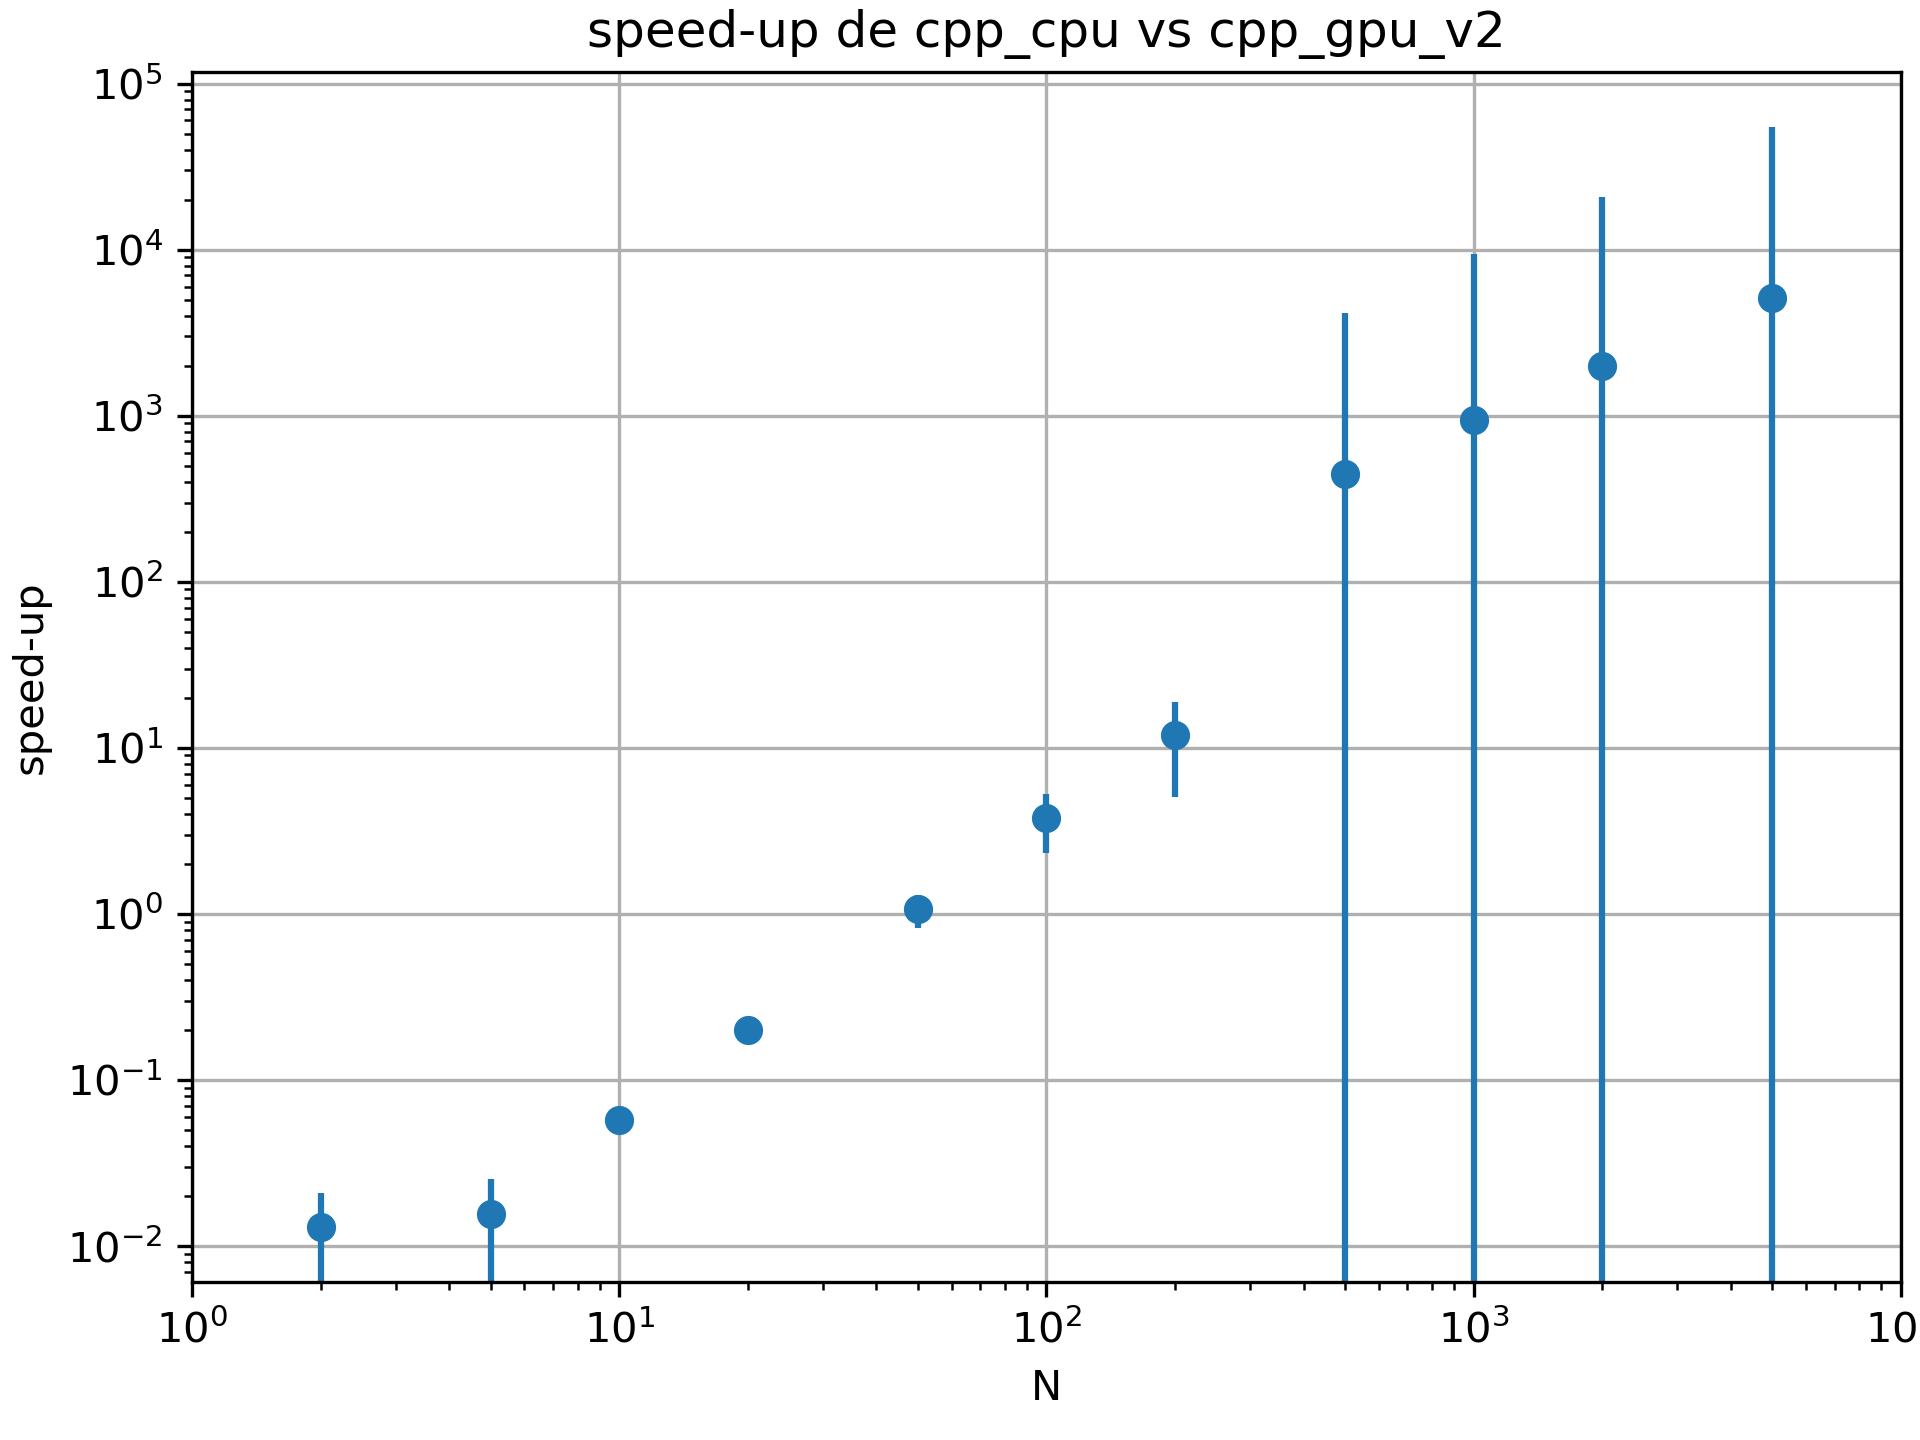
\includegraphics[clip=true,width=\columnwidth]{cpp_cpu_vs_cpp_gpu_v2.png}
    \caption{Gráfico de speed-up respecto a cpp_cpu}
     \label{fig:cpp_cpu_vs_cpp_gpu_v2}
\end{figure}

\begin{figure}[h]
    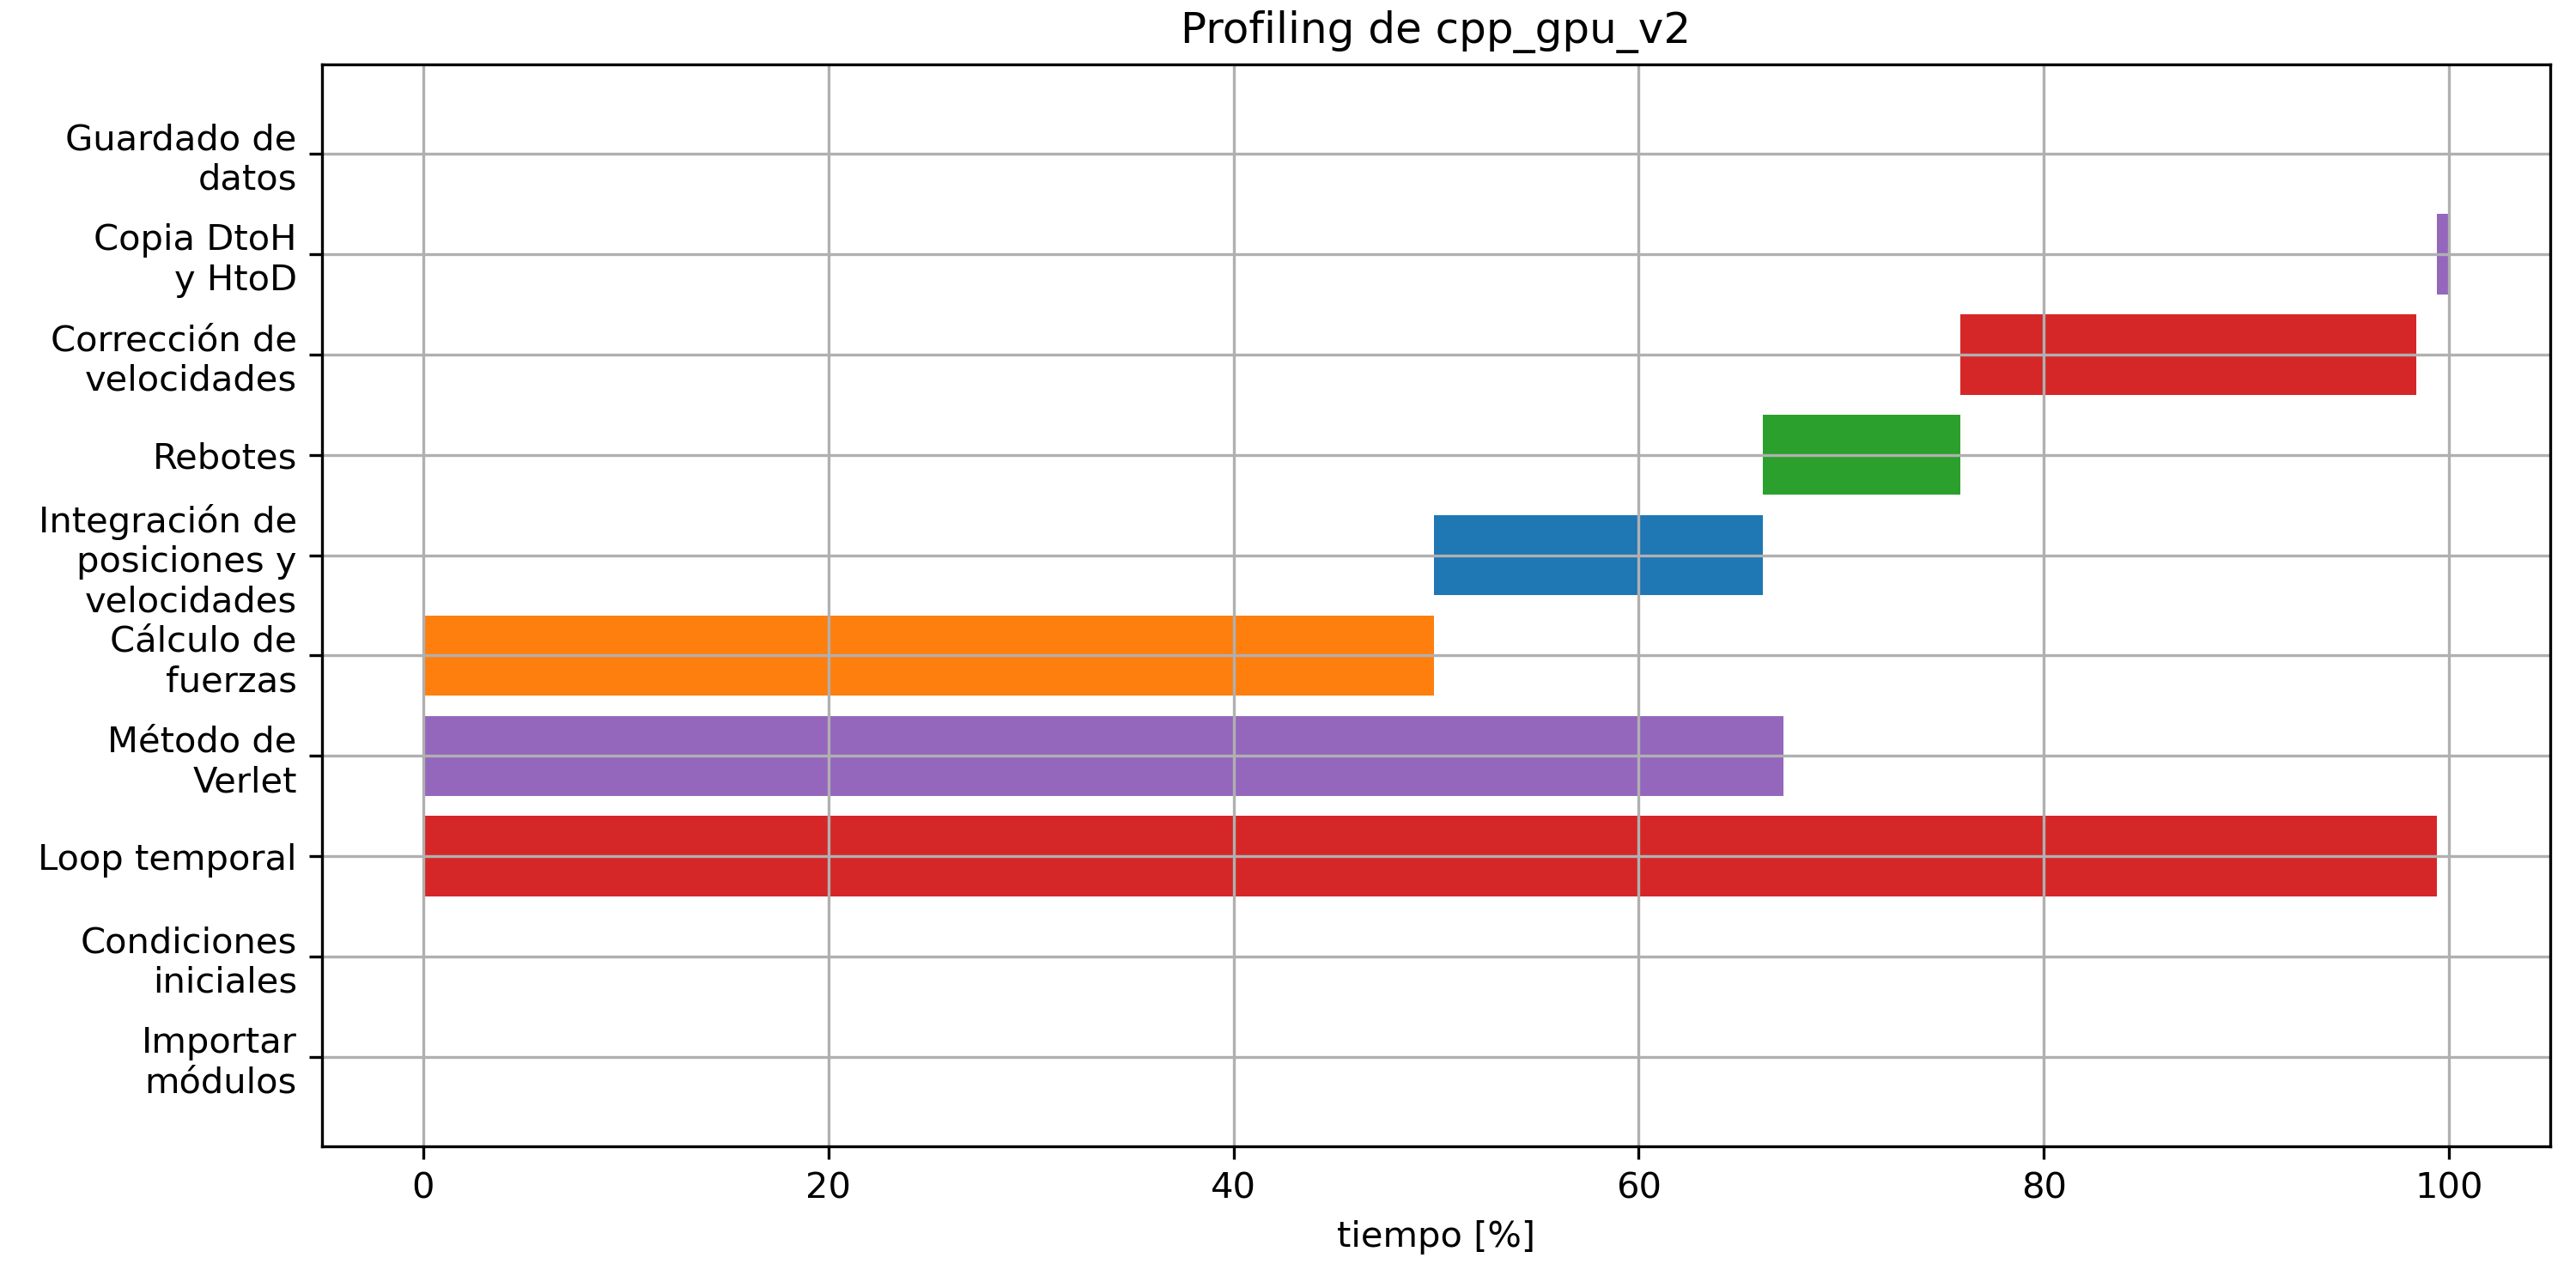
\includegraphics[clip=true,width=\columnwidth]{Profiling de cpp_gpu_v2.png}
    \caption{Profiling}
     \label{fig:Profiling de cpp_gpu_v2}
\end{figure}

\section{Resultados}

-Animación o gráfico de los resultados
\textcolor{red}{Hacer una animación de la densidad radial en el tiempo comparándola con la solución de Bunkin para N grande}



Todo profiling hacerlo con N = 2000

En una CPU con
Información de la CPU:
Nombre: AMD Ryzen 7 4700U with Radeon Graphics
Arquitectura: X86_64
Frecuencia: [1400000000, 0]
Núcleos físicos: 8

py_cpu:

Para hacer profiling:
jupyter nbconvert py_cpu_simulacion_de_particulas.ipynb --to python
python -m cProfile -o py_cpu_simulacion_de_particulas.profile py_cpu_simulacion_de_particulas.py
snakeviz py_cpu_simulacion_de_particulas.profile

Del total
85.15 para hacer el loop temporal
13.83 lo usa el compilador para importar módulos
0.77 para guardar los archivos txt

Del 85.15:
85.10 se usa para el método de Verlet, el restante para los rebotes

Del 85.10:
82.38 se usa para calcular las fuerzas, el restante para integrar posiciones y velocidades

-------------
CPU: AMD Ryzen 7 4700U with Radeon Graphics
Tiempo total: 100

P1 Importar módulos: 13.83
P2 Condiciones iniciales: 0.
P3 Loop temporal: 85.15
S1 Método de Verlet: 85.10
SS1 Cálculo de fuerzas: 82.38
SS2 Integración de posiciones y velocidades: 85.10-82.38
S2 Rebotes: 0.025
S3 Corrección de velocidades: 0.025
P4 Guardado de datos: 0.77
-----------------




py_gpu:
Para hacer profiling:
jupyter nbconvert py_gpu_simulacion_de_particulas.ipynb --to python
python -m cProfile -o py_gpu_simulacion_de_particulas.profile py_gpu_simulacion_de_particulas.py
snakeviz py_gpu_simulacion_de_particulas.profile

Información de la CPU:
Nombre: Intel(R) Xeon(R) CPU @ 2.00GHz
Arquitectura: X86_64
Frecuencia: [2000144000, 0]
Núcleos físicos: 2
Device 0 Name: Tesla T4

cargar librerías: 55.45 %
condiciones iniciales: 24.68%
avanzo_dt: 18.87 %
save_txt: 0.52 %

dentro de avanzo_dt
metodo_Verlet: 2.89%
where: 14.84 % para encontrar dónde el cociente del cálculo de fuerzas se hace nulo
compilación de cupy: 12.44 %
correccion_Temperatura: 0.41%
restante otros procesos


-------------
CPU: Intel(R) Xeon(R) CPU @ 2.00GHz
GPU: Nvidia Tesla T4

P1 Importar módulos: 55.45
P2 Condiciones iniciales: 24.68
P3 Copias HtoD and DtoH: 0.
P4 Loop temporal: 18.87
S1 Método de Verlet: 2.89
SS1 Cálculo de fuerzas: 2.47
SS2 Integración de posiciones y velocidades: 2.89 - 2.47
S2 Rebotes: 14.84
S3 Corrección de velocidades: 0.41
P5 Guardado de datos: 0.52
-------------

¿Cómo hago profiling de un código escrito en C++? Quiero obtener un archivo del tipo .profile



cpp_cpu

Para hacer profiling:

1. Compilar usando la opción-pg
2. Ejecutarlo
g++ -O3 -pg cpp_cpu_funciones.cpp cpp_cpu_simulacion_de_particulas.cpp -o cpp_cpu_simulacion_de_particulas

cpp_cpu_funciones.exe

gprof cpp_cpu_simulacion_de_particulas gmon.out > cpp_cpu_simulacion_de_particulas_profiling.txt


Las pruebas se realizaron en una CPU AMD Phenom II X4 955 con una arquitectura de 64 bits. Esta CPU tiene 4 núcleos, con una frecuencia de reloj de 3.21 GHz.


cpp_gpu_v1

Las pruebas se realizaron en una CPU AMD Phenom II X4 955 con una arquitectura de 64 bits. Esta CPU tiene 4 núcleos, con una frecuencia de reloj de 3.21 GHz.

Además, se empleó una GPU NVIDIA GeForce GTX TITAN X

% GPU Activities

% P1 Importar módulos: 0
% P2 Condiciones iniciales: 0
% P3 Loop temporal: 100 - 0.14-0.13
% S1 Método de Verlet: 100-18.94-1.03-0.14-0.13
% SS1 Cálculo de fuerzas: 77.73
% SS2 Integración de posiciones y velocidades: 1.06 + 0.99
% S2 Rebotes: 1.03
% S3 Corrección de velocidades: 18.94
% P4 Copia DtoH y HtoD: 0.14+0.13
% P5 Guardado de datos: 0

% API Calls

% P1: cudaMalloc 97.46%
% cudaDeviceSynchronize: 1.93 %
% cudaLaunchKernel: 0.37%

cpp_cpu_v2

Las pruebas se realizaron en una CPU AMD Phenom II X4 955 con una arquitectura de 64 bits. Esta CPU tiene 4 núcleos, con una frecuencia de reloj de 3.21 GHz.

Además, se empleó una GPU NVIDIA GeForce GTX TITAN X

% GPU Activities

% P1 Importar módulos: 0
% P2 Condiciones iniciales: 0 
% P3 Loop temporal: 100-0.61
% S1 Método de Verlet: 100-22.53-9.71-0.61
% SS1 Cálculo de fuerzas: 49.89
% SS2 Integración de posiciones y velocidades: 8.75+7.51
% S2 Rebotes: 9.71
% S3 Corrección de velocidades: 22.53
% P4 Copia DtoH y HtoD: 0.61
% P5 Guardado de datos: 0

% API Calls

% P1: cudaMalloc: 99.06
% cudaDeviceSynchronize: 0.32 
% cudaLaunchKernel: 0.38


\bibliography{Chehade_IntroCUDA.bib}

\end{document}





